\documentclass{beamer}
\usepackage[utf8]{inputenc}
\usepackage{graphicx, epsfig}
\usepackage{amsmath,mathrsfs,amsfonts,amssymb}
%\usepackage{subfig}
\usepackage{floatflt}
\usepackage{epic,ecltree}
\usepackage{mathtext}
\usepackage{fancybox}
\usepackage{fancyhdr}
\usepackage{multirow}
\usepackage{enumerate}
\usepackage{epstopdf}
\usepackage{multicol}
\usepackage{algorithm}
\usepackage[noend]{algorithmic}
\def\algorithmicrequire{\textbf{Input:}}
\def\algorithmicensure{\textbf{Output:}}
\usetheme{default}%{Singapore}%{Warsaw}%{Warsaw}%{Darmstadt}
\usecolortheme{default}
\setbeamerfont{title}{size=\Huge}
\setbeamertemplate{footline}[page number]{}
\setbeamerfont{title}{size=\Huge}
\beamertemplatenavigationsymbolsempty

% latin bold lower
\newcommand{\ba}{\mathbf{a}} 
\newcommand{\bc}{\mathbf{c}} 
\newcommand{\be}{\mathbf{e}} 
\newcommand{\bh}{\mathbf{h}} 
\newcommand{\bp}{\mathbf{p}} 
\newcommand{\bt}{\mathbf{t}} 
\newcommand{\bu}{\mathbf{u}} 
\newcommand{\bv}{\mathbf{v}} 
\newcommand{\bw}{\mathbf{w}} 
\newcommand{\bx}{\mathbf{x}} 
\newcommand{\by}{\mathbf{y}} 
\newcommand{\bz}{\mathbf{z}} 

% latin bold upper
\newcommand{\bA}{\mathbf{A}} 
\newcommand{\bC}{\mathbf{C}} 
\newcommand{\bI}{\mathbf{I}} 
\newcommand{\bM}{\mathbf{M}} 
\newcommand{\bT}{\mathbf{T}} 
\newcommand{\bU}{\mathbf{U}} 
\newcommand{\bW}{\mathbf{W}} 
\newcommand{\bX}{\mathbf{X}} 
\newcommand{\bY}{\mathbf{Y}} 
\newcommand{\bZ}{\mathbf{Z}} 

% latin cal upper
\newcommand{\cL}{\mathcal{L}} 
\newcommand{\cN}{\mathcal{N}} 
\newcommand{\cS}{\mathcal{S}} 
\newcommand{\cT}{\mathcal{T}} 
\newcommand{\cW}{\mathcal{W}} 
\newcommand{\cX}{\mathcal{X}} 
\newcommand{\cZ}{\mathcal{Z}} 

% latin cal upper
\newcommand{\bbE}{\mathbb{E}} 
\newcommand{\bbP}{\mathbb{P}} 
\newcommand{\bbR}{\mathbb{R}} 

% greek bold lower
\newcommand{\bepsilon}{\boldsymbol{\epsilon}} 
\newcommand{\btheta}{\boldsymbol{\theta}} 
\newcommand{\blambda}{\boldsymbol{\lambda}} 
\newcommand{\bmu}{\boldsymbol{\mu}} 
\newcommand{\bsigma}{\boldsymbol{\sigma}} 
\newcommand{\bphi}{\boldsymbol{\phi}} 

% greek bold upper
\newcommand{\bSigma}{\boldsymbol{\Sigma}} 

\DeclareMathOperator*{\argmin}{arg\,min}
\DeclareMathOperator*{\argmax}{arg\,max}

\newcommand{\createdgmtitle}[1]{\title[\hbox to 56mm{Deep Generative Models  \hfill\insertframenumber\,/\,\inserttotalframenumber}]
	{\vspace{1cm} \\ Deep Generative Models \\ Lecture #1 \\ \vspace{-0.5cm}}
	\author{Roman Isachenko \\ \vspace{-0.5cm}}
	\institute{
\includegraphics[width=3cm]{../utils/ozonmasterslogo}
	\\Ozon Masters
	}
	\date{Spring, 2021}
}

\newcommand\myfootnote[1]{%
  \tikz[remember picture,overlay]
  \draw (current page.south west) +(1in + \oddsidemargin,0.5em)
  node[anchor=south west,inner sep=0pt]{\parbox{\textwidth}{%
      \rlap{\rule{10em}{0.4pt}}\raggedright\scriptsize#1}};}

\newcommand\myfootnotewithlink[2]{%
  \tikz[remember picture,overlay]
  \draw (current page.south west) +(1in + \oddsidemargin,0.5em)
  node[anchor=south west,inner sep=0pt]{\parbox{\textwidth}{%
      \rlap{\rule{10em}{0.4pt}}\raggedright\scriptsize\href{#1}{\textit{#2}}}};}
\createdgmtitle{10}
%--------------------------------------------------------------------------------
\begin{document}
%--------------------------------------------------------------------------------
\begin{frame}
%\thispagestyle{empty}
\titlepage
\end{frame}
%=======
\begin{frame}{Evaluation of likelihood-free models}
	How to evaluate generative models?
	\begin{block}{Likelihood-based models}
		\begin{itemize}
			\item Split data to train/val/test.
			\item Fit model on the train part.
			\item Tune hyperparameters on the validation part.
			\item Evaluate generalization by reporting likelihoods on the test set.
		\end{itemize}
	\end{block}
	\begin{block}{Not all models have tractable likelihoods}
		\begin{itemize}
			\item VAE: compare ELBO values.
			\item GAN: ???
		\end{itemize}
	\end{block}
\end{frame}
%=======
\begin{frame}{Evaluation of likelihood-free models}
	Let take some pretrained image classification model to get the conditional label distribution $p(y | \bx)$ (e.g. ImageNet classifier).
	\begin{block}{What do we want from samples?}
		\begin{itemize}
			\item \textbf{Sharpness}
			\begin{figure}
				\centering
				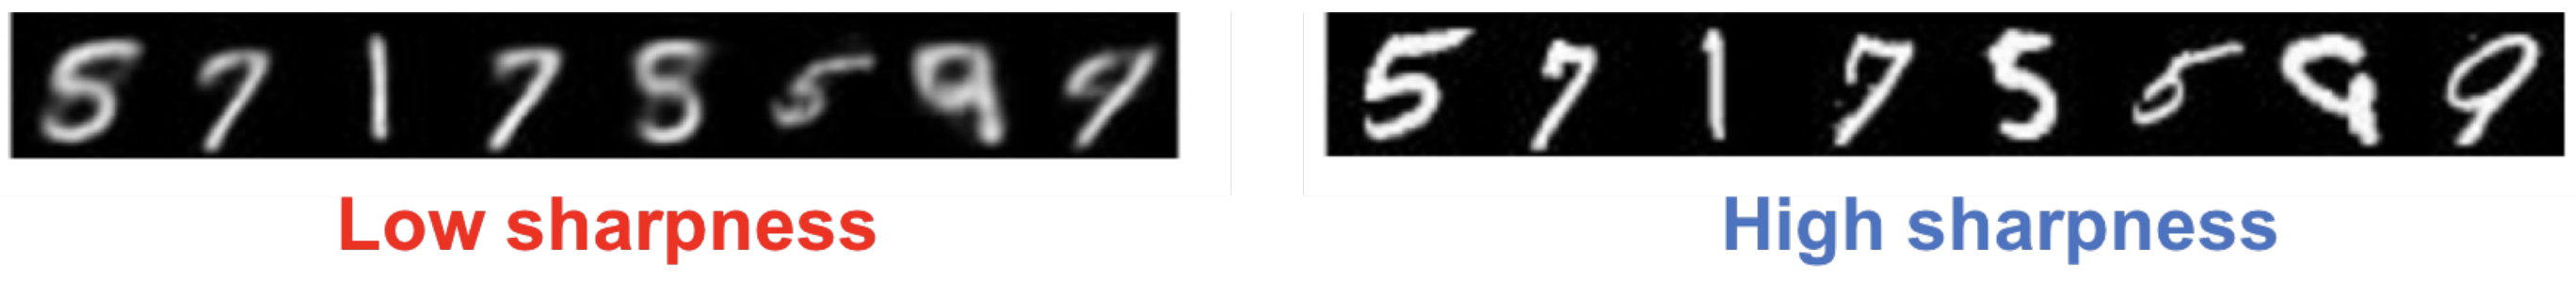
\includegraphics[width=0.9\linewidth]{figs/sharpness}
			\end{figure}
			The conditional distribution $p(y | \bx)$ should have low entropy (each image $\bx$ should have distinctly recognizable object).
			\item \textbf{Diversity}
			\begin{figure}
				\centering
				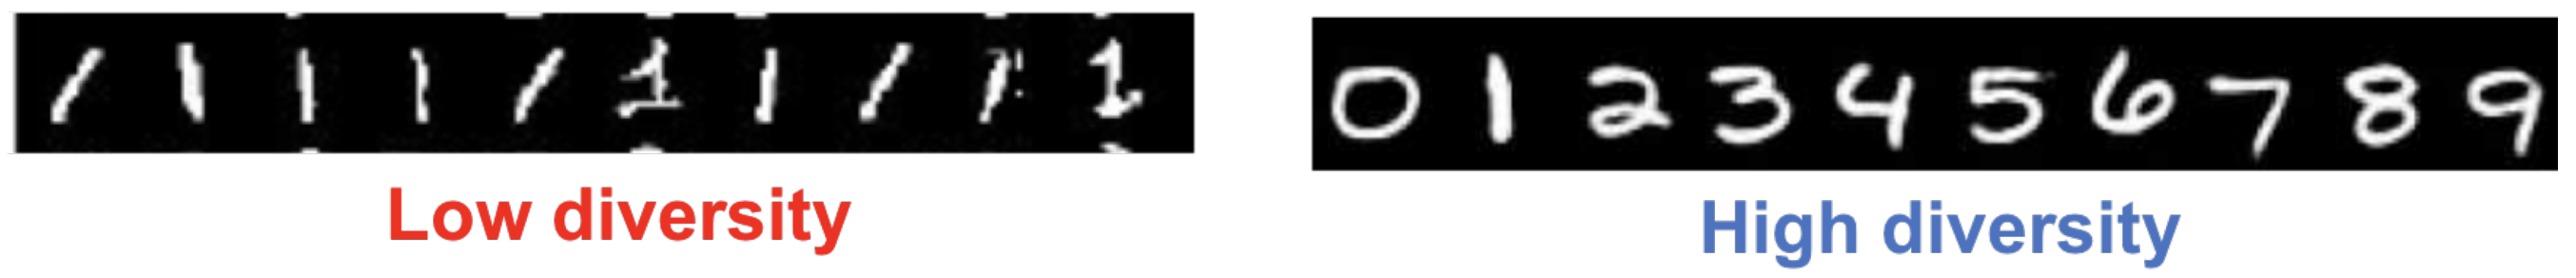
\includegraphics[width=0.9\linewidth]{figs/diversity}
			\end{figure}
			The marginal distribution $p(y) = \int p(y | \bx) p(\bx) d \bx$ should have high entropy (there should be as many classes generated as possible).
		\end{itemize}
	\end{block}
	\vfill
	\hrule\medskip 
	{\scriptsize \href{https://deepgenerativemodels.github.io}{https://deepgenerativemodels.github.io}}
\end{frame}
%=======
\begin{frame}{Evaluation of likelihood-free models}
	\begin{block}{What do we want from samples?}
		\begin{itemize}
			\item \textbf{Sharpness.}
			The conditional distribution $p(y | \bx)$ should have low entropy (each image $\bx$ should have distinctly recognizable object).
			\item \textbf{Diversity.}
			The marginal distribution $p(y) = \int p(y | \bx) p(\bx) d \bx$ should have high entropy (there should be as many classes generated as possible).
		\end{itemize}
	\end{block}
	\begin{figure}
		\centering
		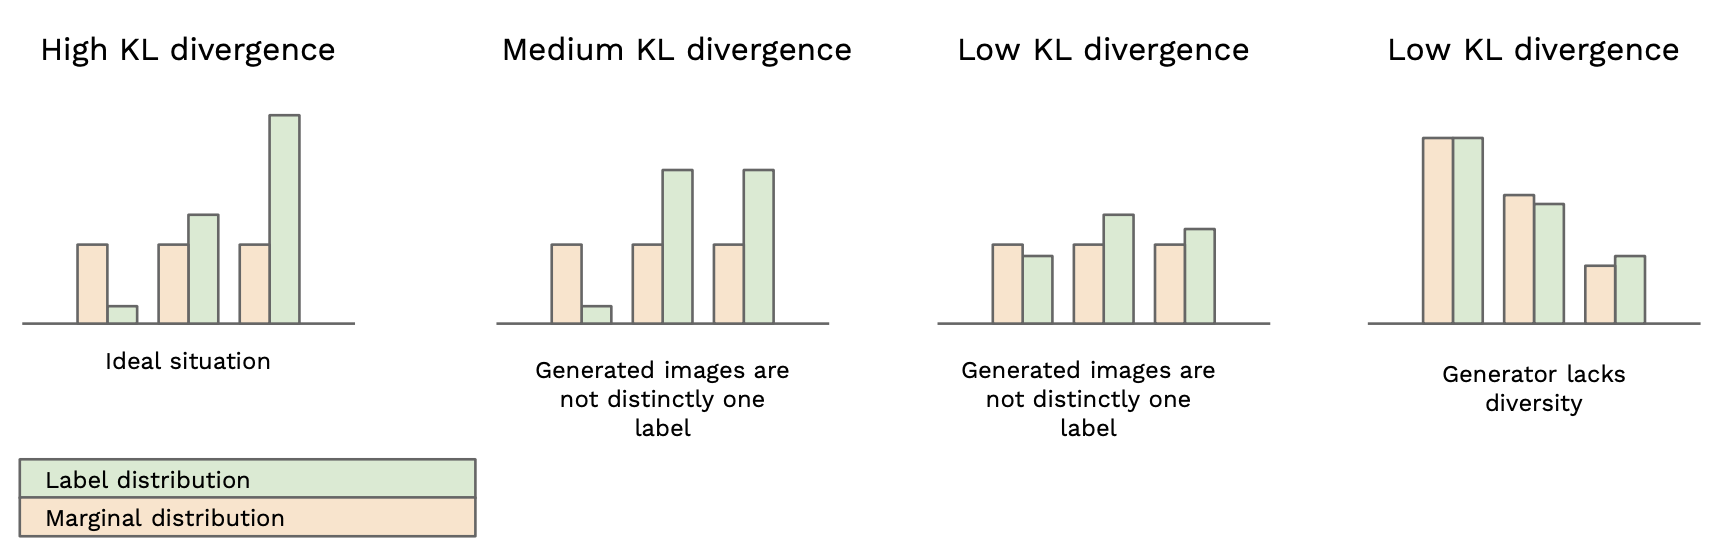
\includegraphics[width=1.0\linewidth]{figs/is_toy}
	\end{figure}
	\vfill
	\hrule\medskip 
	{\scriptsize \href{https://medium.com/octavian-ai/a-simple-explanation-of-the-inception-score-372dff6a8c7a}{https://medium.com/octavian-ai/a-simple-explanation-of-the-inception-score-372dff6a8c7a}}
\end{frame}
%=======
\begin{frame}{Evaluation of likelihood-free models}
		\begin{block}{What do we want from samples?}
		\begin{itemize}
			\item Sharpness $\Rightarrow$ low $H(y | \bx) = - \sum_{y} \int_{\bx} p(y, \bx) \log p(y | \bx) d\bx$.
			\item Diversity $\Rightarrow$ high $H(y)  = - \sum_{y} p(y) \log p(y)$.
		\end{itemize}
	\end{block}
	\begin{block}{Inception Score}
		\vspace{-0.3cm}
		\footnotesize
		\begin{align*}
			IS &= \exp(H(y) - H(y | \bx)) \\ 
			&= \exp \left( - \sum_{y} p(y) \log p(y) + \sum_{y} \int_{\bx} p(y, \bx) \log p(y | \bx) d\bx\right) \\
			&= \exp \left( \sum_{y} \int_{\bx} p(y, \bx) \log \frac{p(y | \bx)}{p(y)} d\bx\right) \\ 
			&= \exp \left( \bbE_{\bx} \sum_{y} p(y | \bx) \log \frac{p(y | \bx)}{p(y)} \right) = \exp \left( \bbE_{\bx} KL(p(y | \bx) || p(y)) \right)
		\end{align*}
	\end{block}
	\vfill
	\hrule\medskip 
	{\scriptsize \href{https://arxiv.org/abs/1606.03498}{https://arxiv.org/abs/1606.03498}}
\end{frame}
%=======
\begin{frame}{Evaluation of likelihood-free models}
	\begin{block}{Inception Score}
		\vspace{-0.1cm}
		\[
			IS =  \exp \left( \bbE_{\bx} KL(p(y | \bx) || p(y)) \right)
		\]
		\vspace{-0.1cm}
	\end{block}
	\begin{block}{IS limitations}
		\begin{itemize}
			\item Inception score depends on the quality of the pretrained classifier $p(y | \bx)$.
			\item If generator produces images with a different set of labels from the classifier training set, IS will be low.
			\item If the generator produces one image per class, the IS will be perfect (there is no measure of intra-class diversity).
			\item IS only require samples from the generator and do not take into account the desired data distribution $\pi(\bx)$ directly (only implicitly via a classifier).
		\end{itemize}
	\end{block}
	\vfill
	\hrule\medskip 
	{\scriptsize \href{https://arxiv.org/abs/1801.01973}{https://arxiv.org/abs/1801.01973}}
\end{frame}
%=======
\begin{frame}{Evaluation of likelihood-free models}
	\begin{block}{Theorem}
		If $\pi(\bx)$ and $p(\bx | \btheta)$ has moment generation functions then
		\[
			\pi(\bx) = p(\bx | \btheta) \, \Leftrightarrow \, \bbE_{\pi} \bx^k = \bbE_{p} \bx^k, \quad \forall k \geq 1.
		\]
	\end{block}
	This is intractable to calculate all moments.
	\begin{block}{Frechet Inception Distance}
		\vspace{-0.1cm}
		\[
			D^2 (\pi, p) = \| \mathbf{m}_{\pi} - \mathbf{m}_{p}\|_2^2 + \text{Tr} \left( \bC_{\pi} + \bC_p - 2 \sqrt{\bC_{\pi} \bC_p} \right)
		\]
	\end{block}
	\begin{itemize}
		\item $\mathbf{m}_{\pi}$, $\bC_{\pi} $ are mean vector and covariance matrix of feature representations for real samples from $\pi(\bx)$
		\item $\mathbf{m}_{p}$, $\bC_p$ are mean vector and covariance matrix of feature representations for generated samples from $p(\bx | \btheta)$.
		\item Representations are outputs of intermediate layer from pretrained classification model.
	\end{itemize} 

	\vfill
	\hrule\medskip 
	{\scriptsize \href{https://arxiv.org/abs/1706.08500}{https://arxiv.org/abs/1706.08500}}
\end{frame}
%=======
\begin{frame}{Evaluation of likelihood-free models}
	\begin{figure}
		\centering
		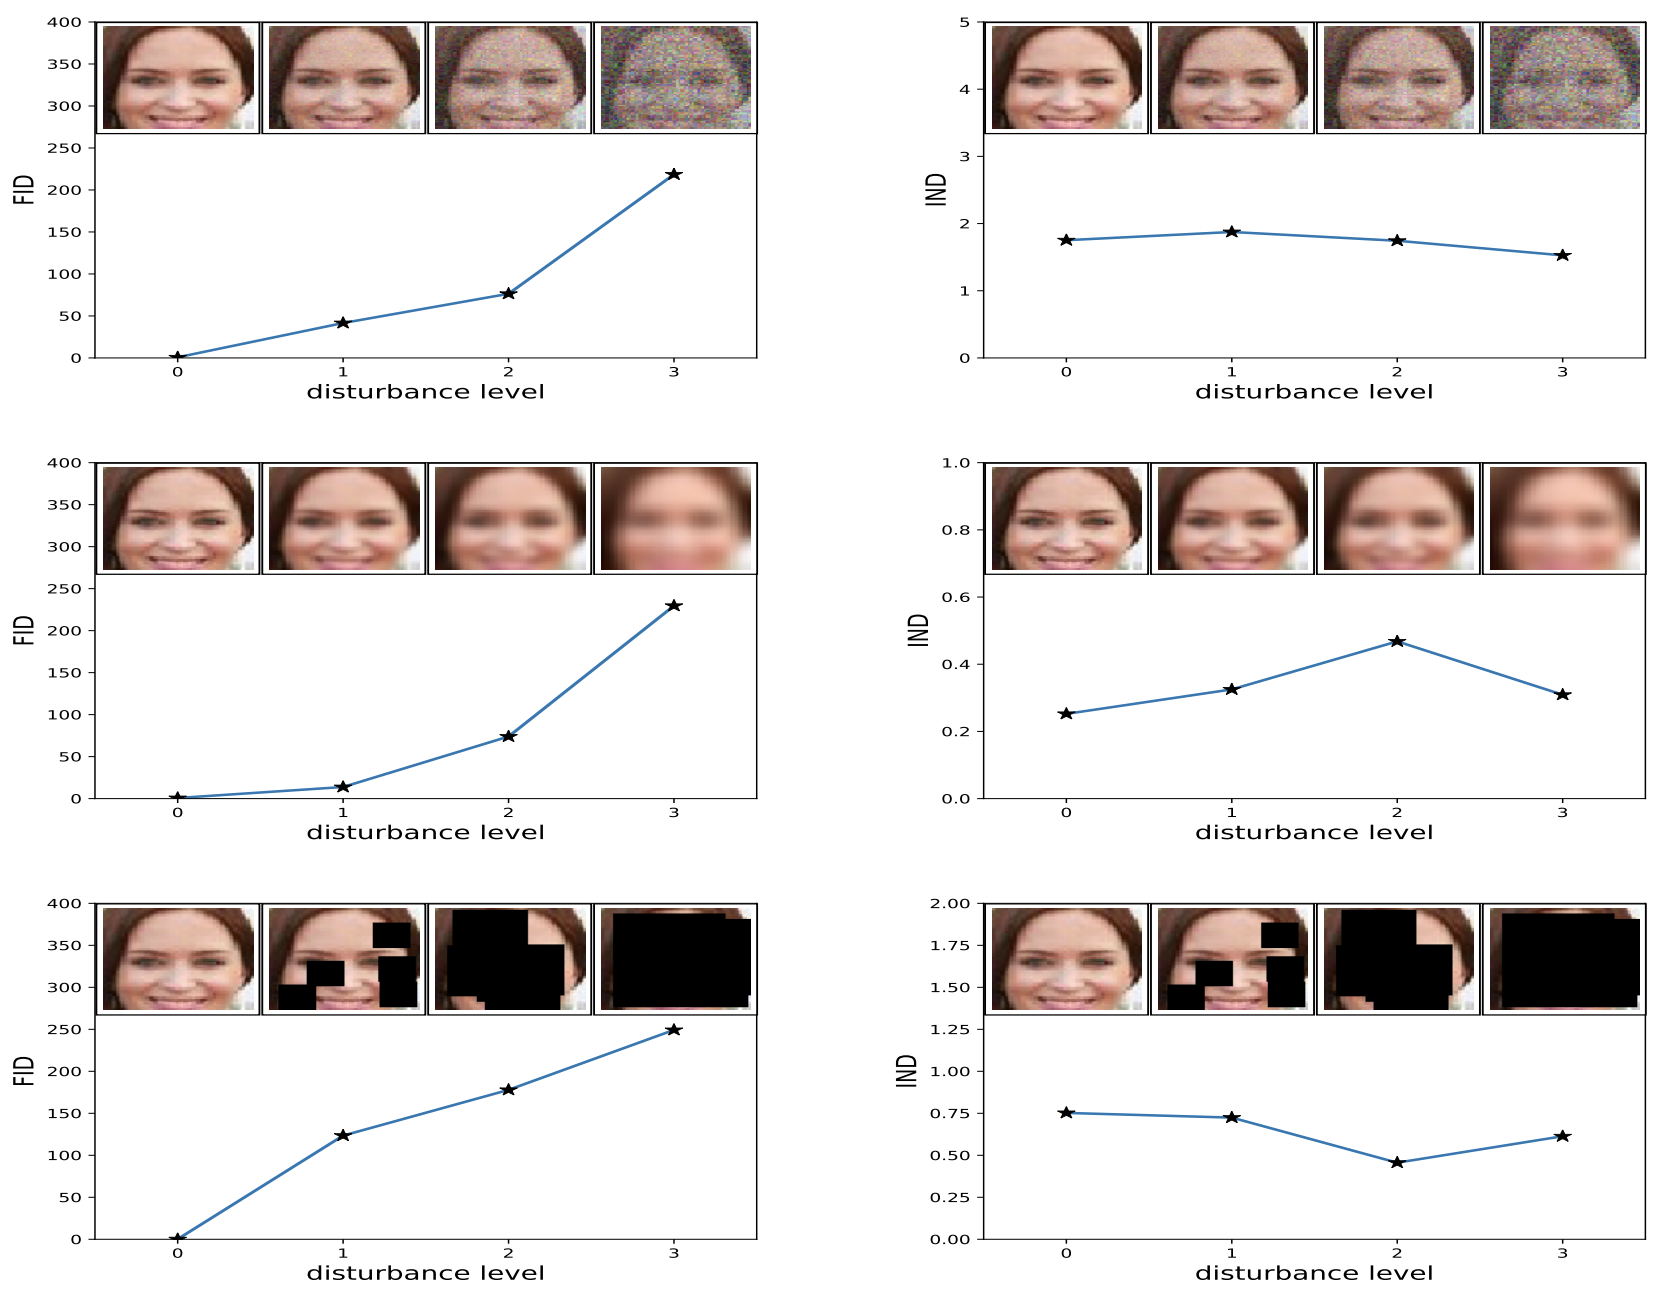
\includegraphics[width=0.9\linewidth]{figs/fid_results}
	\end{figure}
	\vfill
	\hrule\medskip 
	{\scriptsize \href{https://arxiv.org/abs/1706.08500}{https://arxiv.org/abs/1706.08500}}
\end{frame}
%=======
\begin{frame}{Evaluation of likelihood-free models}
	\begin{block}{Frechet Inception Distance}
		\vspace{-0.1cm}
		\[
		D^2 (\pi, p) = \| \mathbf{m}_{\pi} - \mathbf{m}_{p}\|_2^2 + \text{Tr} \left( \bC_{\pi} + \bC_p - 2 \sqrt{\bC_{\pi} \bC_p} \right)
		\]
	\end{block}
	\begin{block}{FID limitations}
		\begin{itemize}
			\item FID depends on the pretrained classification model.
			\item FID needs a large samples  size for evaluation.
			\item Calculation of FID is slow.
			\item FID extimates only two sample moments.
		\end{itemize}
	\end{block}
	\vspace{2cm}

	\vfill
	\hrule\medskip 
	{\scriptsize \href{https://arxiv.org/abs/1706.08500}{https://arxiv.org/abs/1706.08500}}
\end{frame}
%=======
\begin{frame}{Summary}
	\begin{itemize}
		\item Wasserstein GAN uses Kantorovich-Rubinstein duality to estimate Wasserstein distance.
		\item Gradient Penalty proposes the regularizer to enforce Lipschitzness.
		\item Spectral normalization is a weight normalization technique to enforce Lipshitzness.
		\item f-divergence family is a unified framework for divergence minimization.
		\item Inception Score and Frechet Inception Distance are the common metrics for GAN evaluation.
	\end{itemize}
\end{frame}
%=======
\begin{frame}{Evolution of GANs}
	\begin{figure}
		\centering
		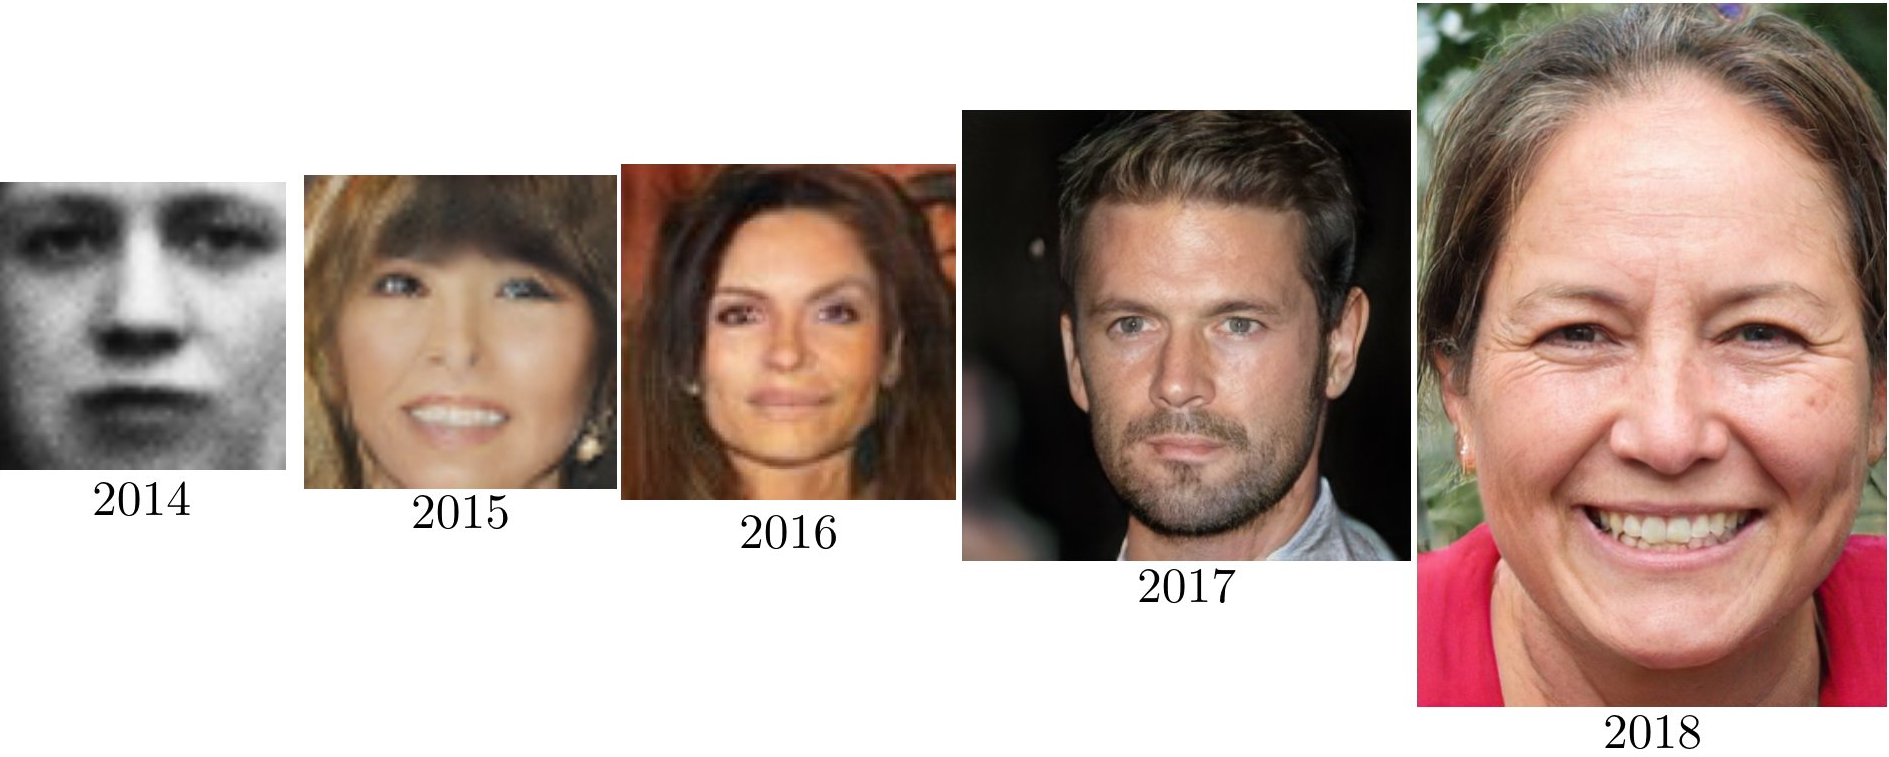
\includegraphics[width=\linewidth]{figs/gan_evolution}
	\end{figure}
	\begin{itemize}
		\item \textbf{Vanilla GAN} \href{https://arxiv.org/abs/1406.2661}{https://arxiv.org/abs/1406.2661}
		\item \textbf{DCGAN} \href{https://arxiv.org/abs/1511.06434}{https://arxiv.org/abs/1511.06434}
		\item \textbf{CoGAN} \href{https://arxiv.org/abs/1606.07536}{https://arxiv.org/abs/1606.07536}
		\item \textbf{ProGAN} \href{https://arxiv.org/abs/1710.10196}{https://arxiv.org/abs/1710.10196} 
		\item \textbf{StyleGAN} \href{https://arxiv.org/abs/1812.04948}{https://arxiv.org/abs/1812.04948}
	\end{itemize}
\end{frame}
%=======
\begin{frame}{Self-Attention GAN}
	\begin{itemize}
		\item Convolutional layers process the information in a local neighborhood.
		\item Using convolutional layers alone is computationally inefficient for modeling long-range dependencies in images.
	\end{itemize}
	\begin{figure}
		\centering
		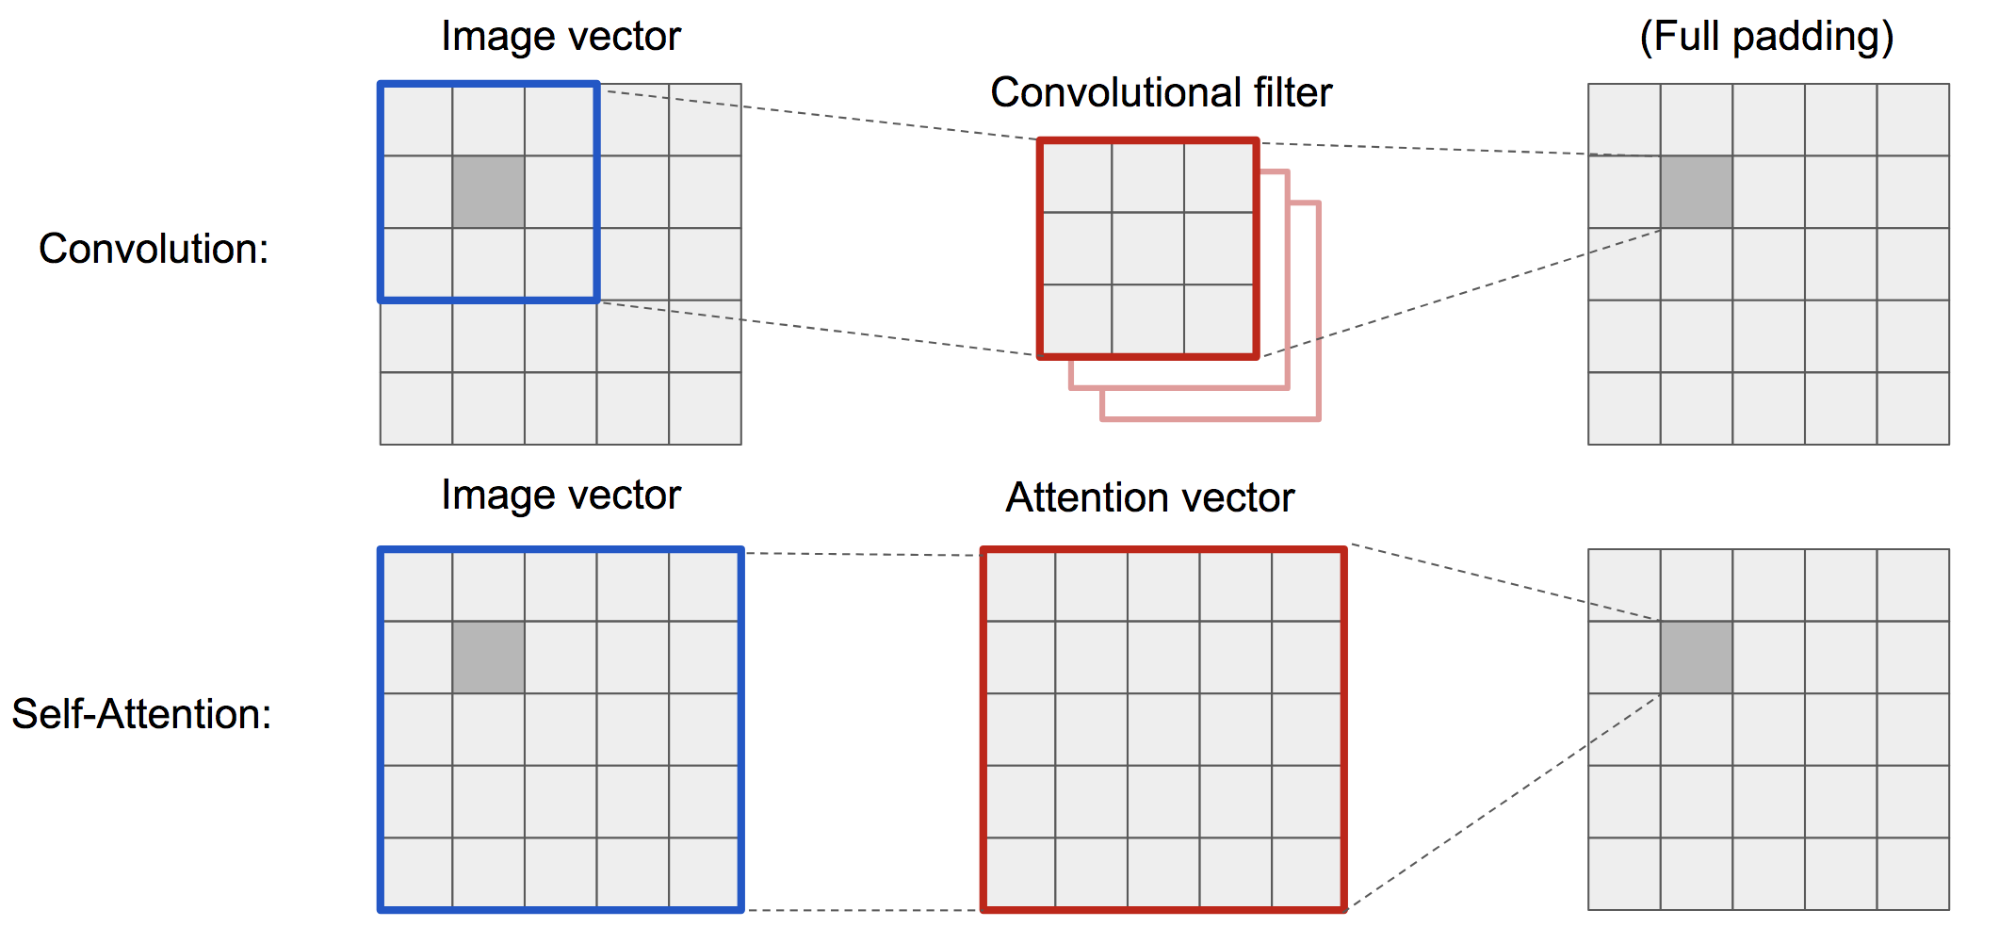
\includegraphics[width=0.9\linewidth]{figs/conv-vs-sa}
	\end{figure}
	\vfill
	\hrule\medskip 
	{\scriptsize \href{https://lilianweng.github.io/lil-log/2018/06/24/attention-attention.html}{https://lilianweng.github.io/lil-log/2018/06/24/attention-attention.html}}
\end{frame}
%=======
\begin{frame}{Self-Attention GAN}
	\begin{figure}
		\centering
		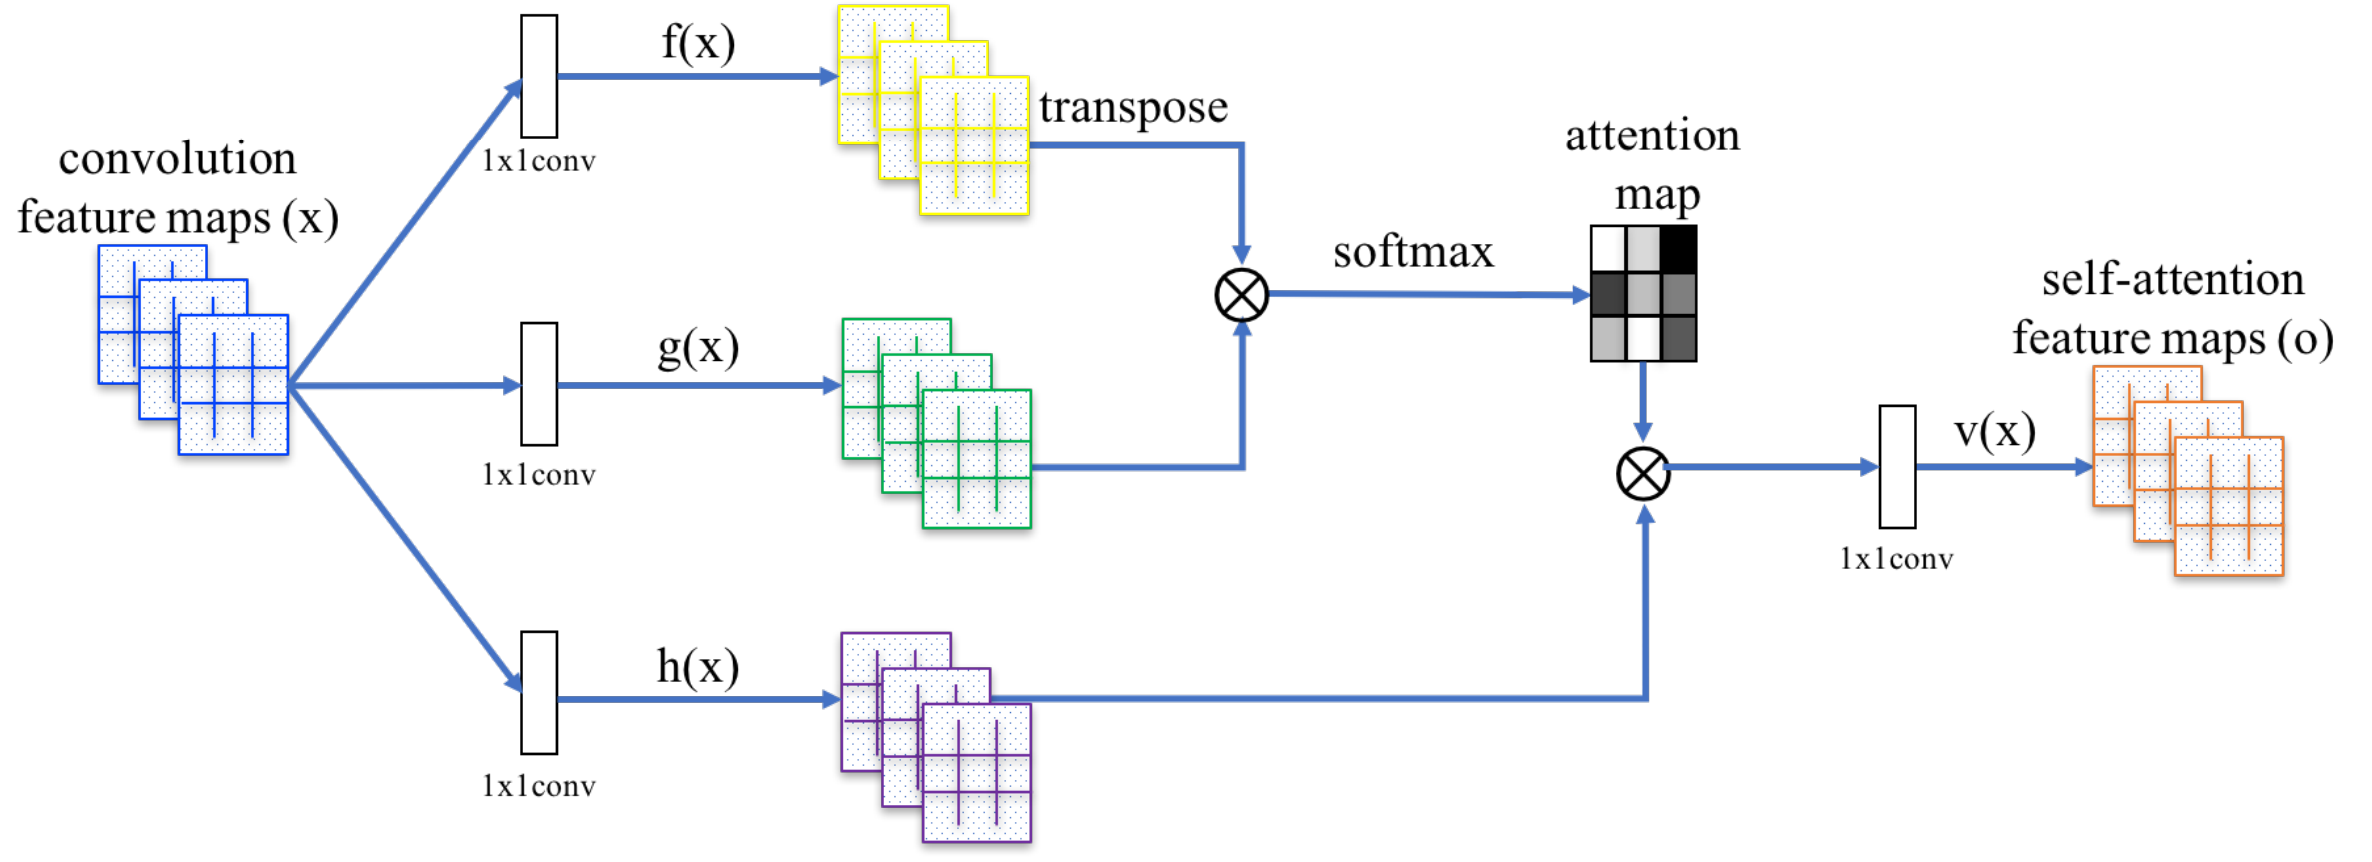
\includegraphics[width=0.9\linewidth]{figs/self-attention}
	\end{figure}
	\vspace{-0.2cm}
	\begin{itemize}
		\item $\bx$ -- feature vector for one feature location.
		\item $N$ -- number of feature locations.
	\end{itemize}
	\vspace{0.5cm}
	\[
		\mathbf{f}(\bx) = \bW_f(\bx), \quad \mathbf{g}(\bx) = \bW_g(\bx), \quad \mathbf{h}(\bx) = \bW_h(\bx), \quad \mathbf{v}(\bx) = \bW_v(\bx)
	\]
	\[
		s_{ij} = \mathbf{f}(\bx_i)^T \mathbf{g}(\bx_j), \quad a_{ij} = \frac{\exp{s_{ij}}}{\sum_{i=1}^N \exp{s_{ij}}}, \quad \textbf{o}_j = \textbf{v}\left( \sum_{i=1}^N a_{ij} \mathbf{h}(\bx_i) \right)
	\]
	\vfill
	\hrule\medskip 
	{\scriptsize \href{https://arxiv.org/abs/1805.08318}{https://arxiv.org/abs/1805.08318}}
\end{frame}
%=======
\begin{frame}{Self-Attention GAN}
	\begin{block}{Technical Details}
		\begin{itemize}
			\item Hinge loss for training.
			\item Spectral Normalization in both the generator and the discriminator.
			\item Separate learning rates for the generator and the discriminator.
		\end{itemize}
	\end{block}
	\begin{figure}
		\centering
		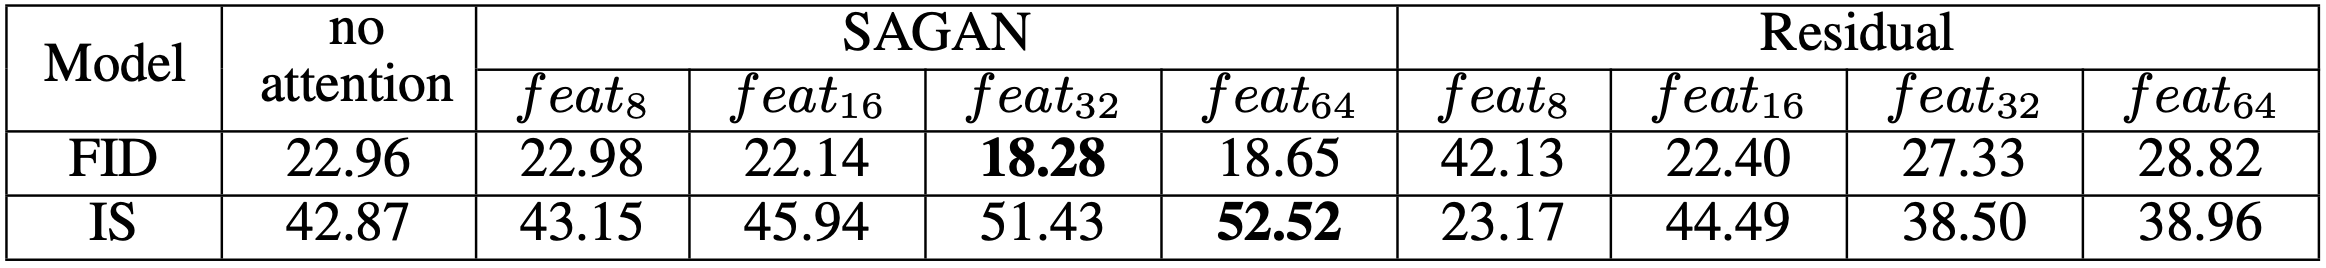
\includegraphics[width=\linewidth]{figs/sa_results1}
	\end{figure}
	\begin{figure}
		\centering
		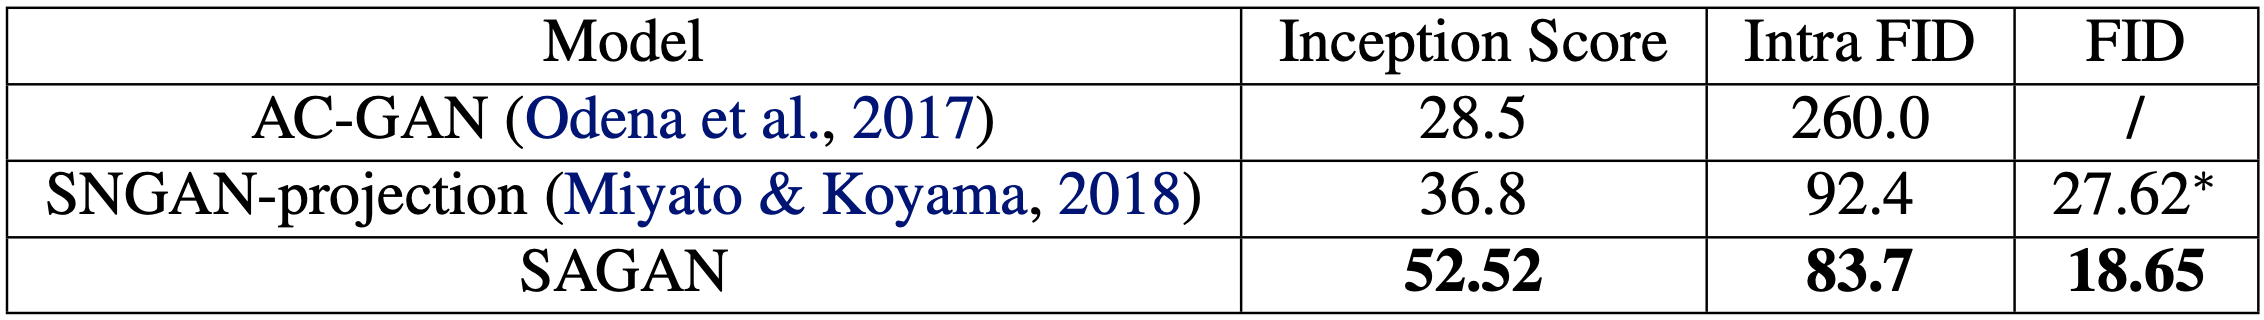
\includegraphics[width=\linewidth]{figs/sa_results2}
	\end{figure}
	\vfill
	\hrule\medskip 
	{\scriptsize \href{https://arxiv.org/abs/1805.08318}{https://arxiv.org/abs/1805.08318}}
\end{frame}
%=======
\begin{frame}{Self-Attention GAN}
	\begin{block}{Visualization of attention maps}
		\begin{figure}
			\centering
			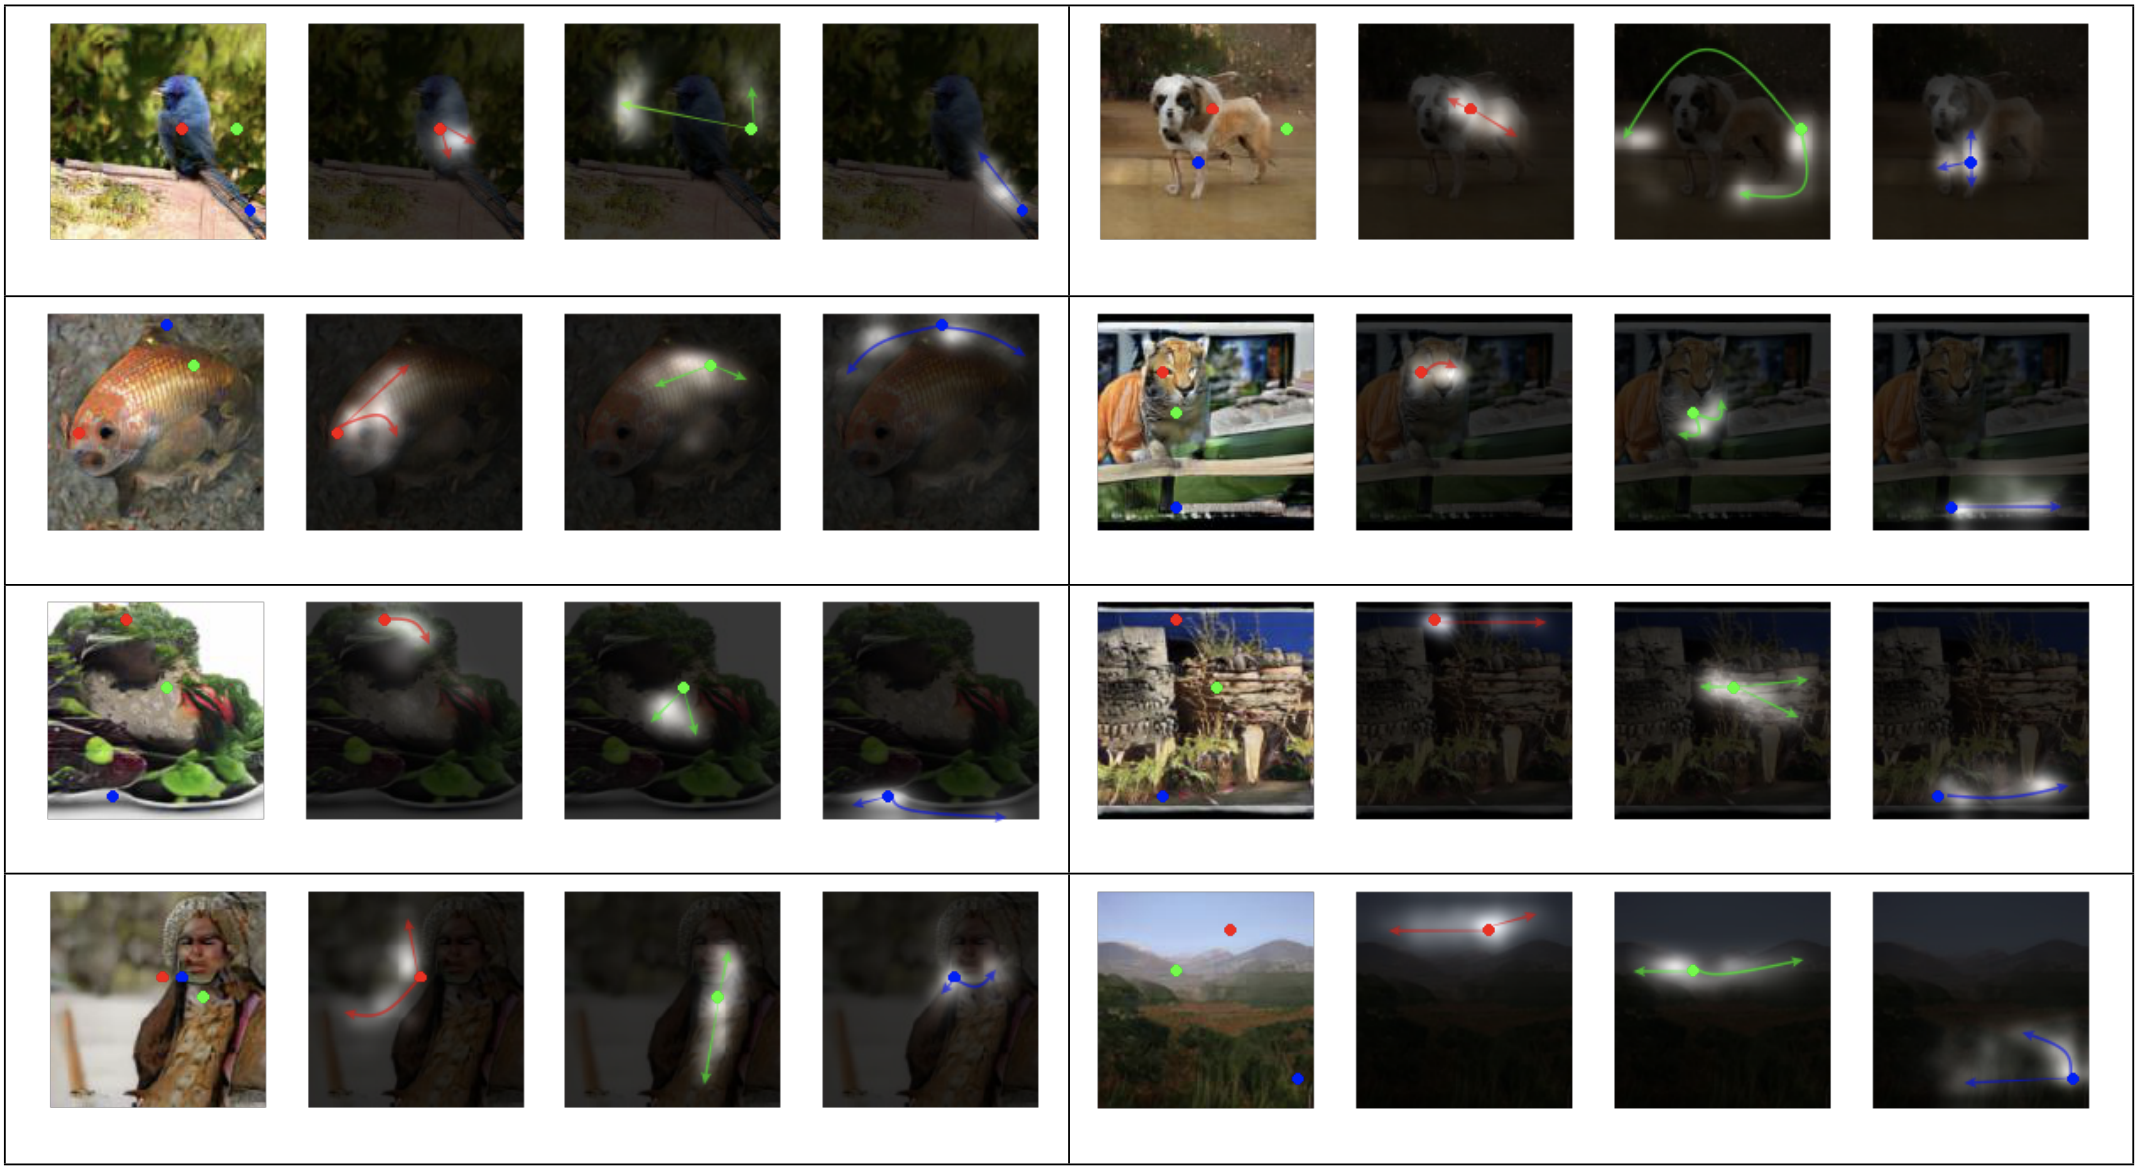
\includegraphics[width=\linewidth]{figs/sa_maps}
		\end{figure}
	\end{block}
	\vfill
	\hrule\medskip 
	{\scriptsize \href{https://arxiv.org/abs/1805.08318}{https://arxiv.org/abs/1805.08318}}
\end{frame}
%=======
\begin{frame}{BigGAN}
	\begin{block}{Model description}
		\begin{itemize}
			\item Self-Attention GAN baseline.
			\item Class-conditional generator.
			\item Increasing batch size gives tremendous benefit (allows to cover more modes).
			\item Increasing model size is helpful (wider helps as much as deeper).
			\item Hinge loss for training.
			\item Orthogonal regularization for smoothness the generator output.
			\item Truncation trick for balancing between diversity and fidelity.
		\end{itemize}
	\end{block}
	\vspace{0.5cm}

	\vfill
	\hrule\medskip 
	{\scriptsize \href{https://arxiv.org/abs/1809.11096}{https://arxiv.org/abs/1809.11096}}
\end{frame}
%=======
\begin{frame}{BigGAN}
	\begin{itemize}
		\item \textbf{Orthogonal regularization}
		\[
		\| \bW^T \bW - \bI \|^2 \quad \Rightarrow \| \bW^T \bW - \text{diag}(\bW^T \bW) \|^2
		\]
		\item \textbf{Truncation trick.} Coordinates of samples $\bz \sim \cN(0, \bI)$ which fall outside a predefined range are resampled to fall inside that range.
	\end{itemize}
	\begin{figure}
		\centering
		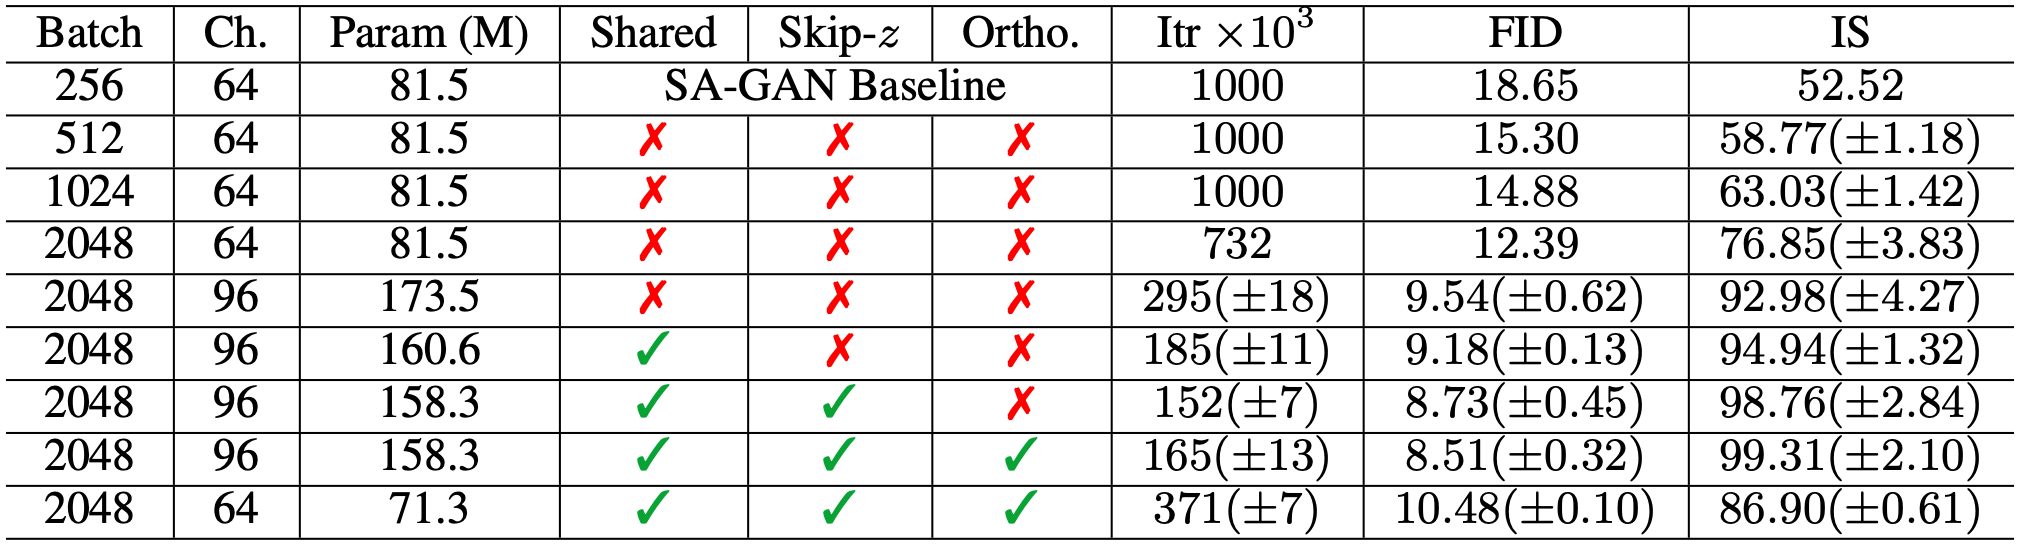
\includegraphics[width=\linewidth]{figs/biggan_results}
	\end{figure}
	\vfill
	\hrule\medskip 
	{\scriptsize \href{https://arxiv.org/abs/1809.11096}{https://arxiv.org/abs/1809.11096}}
\end{frame}
%=======
\begin{frame}{BigGAN}
	\begin{block}{Samples (512x512)}
		\begin{figure}
			\centering
			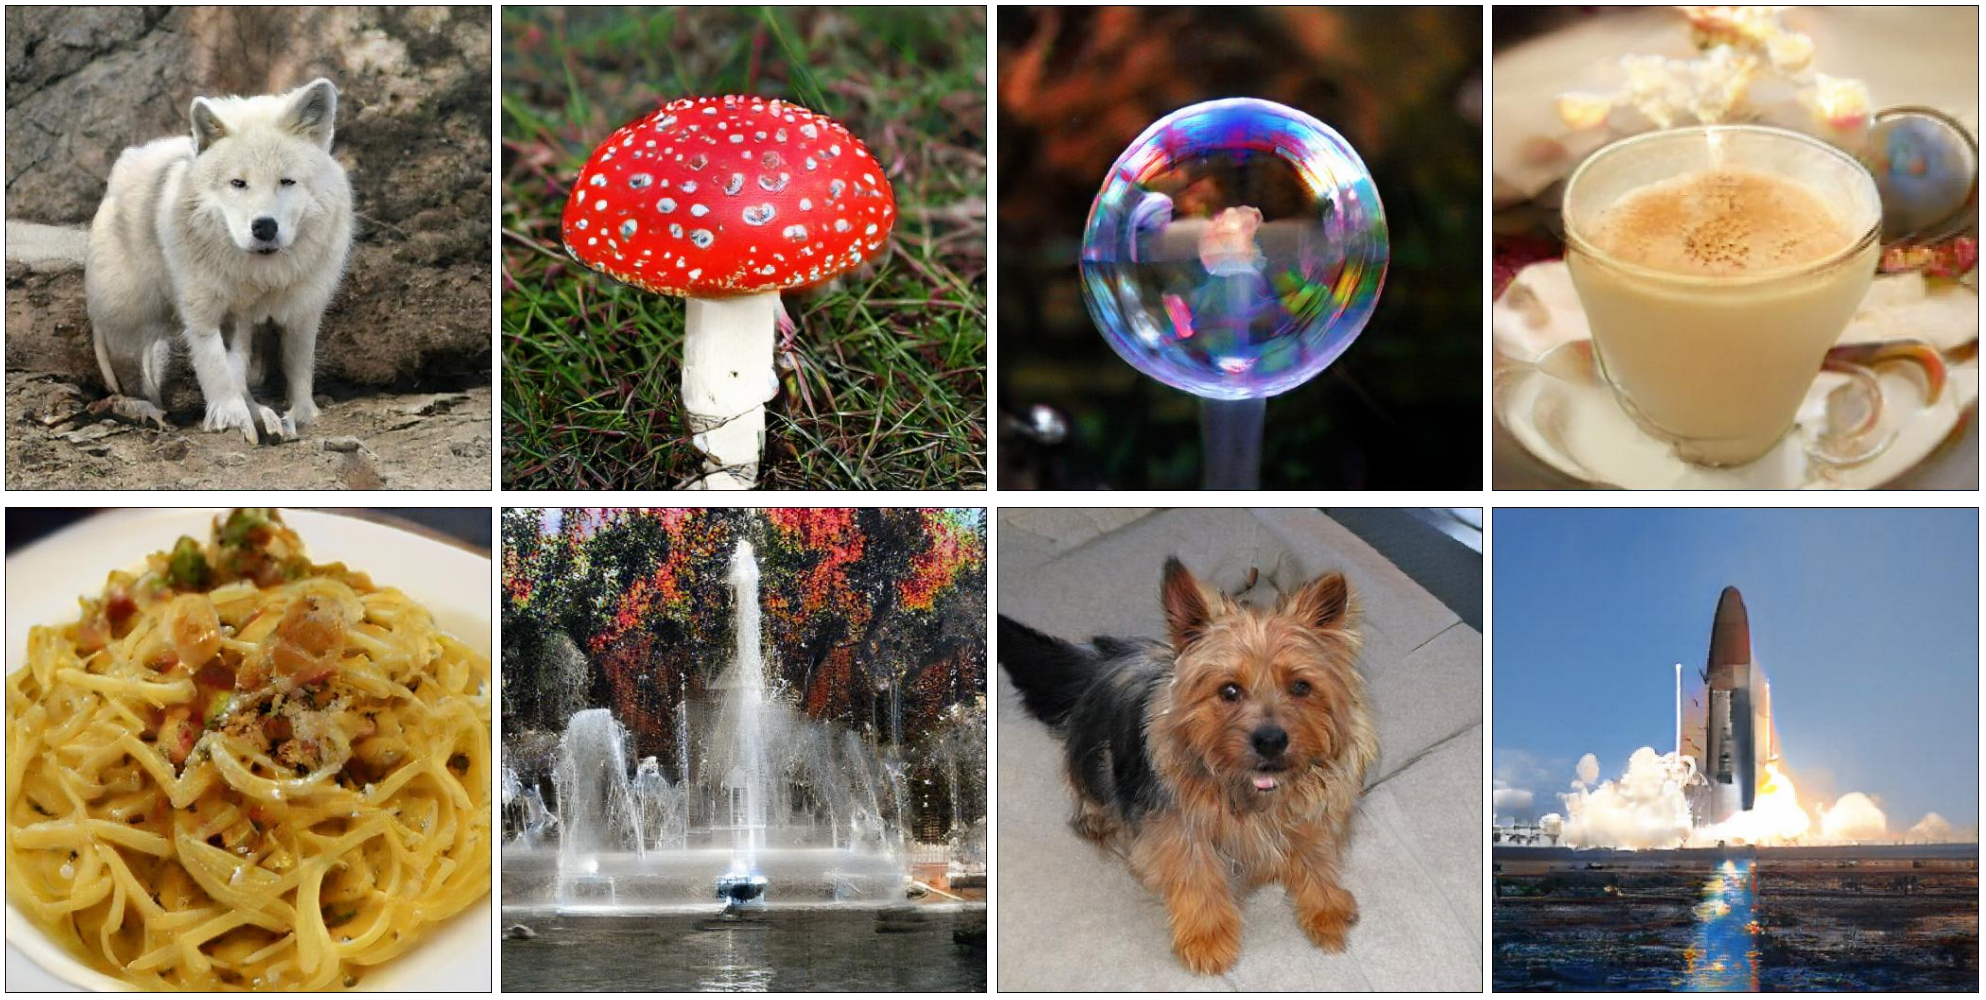
\includegraphics[width=\linewidth]{figs/biggan_samples}
		\end{figure}
	\end{block}
	\vfill
	\hrule\medskip 
	{\scriptsize \href{https://arxiv.org/abs/1809.11096}{https://arxiv.org/abs/1809.11096}}
\end{frame}
%=======
\begin{frame}{BigGAN}
	\begin{block}{Interpolations}
		\begin{figure}
			\centering
			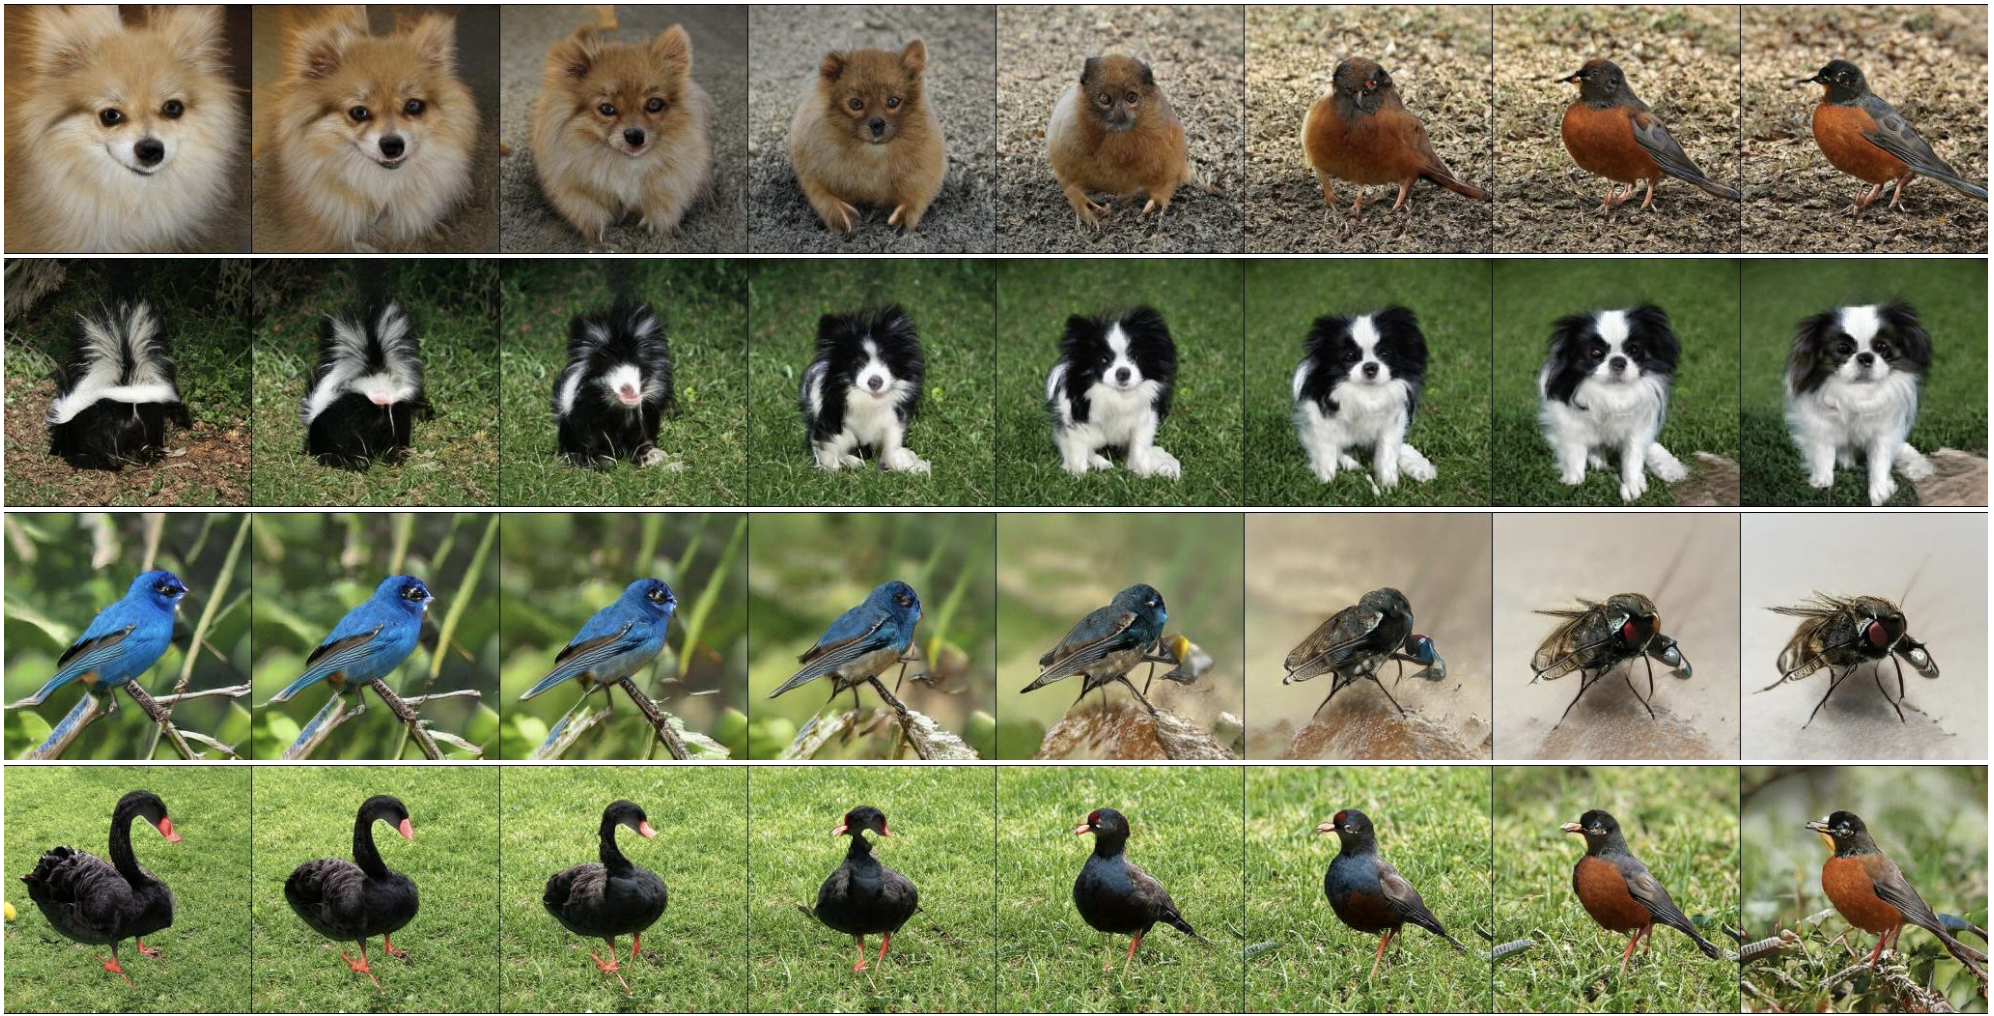
\includegraphics[width=\linewidth]{figs/biggan_interpolations}
		\end{figure}
	\end{block}
	\vfill
	\hrule\medskip 
	{\scriptsize \href{https://arxiv.org/abs/1809.11096}{https://arxiv.org/abs/1809.11096}}
\end{frame}
%=======
\begin{frame}{Progressive Growing GAN}
	\begin{block}{Problems with HR image generation}
		\begin{itemize}
			\item Disjoint manifolds $\Rightarrow$ gradient problem.
			\item Small minibatch $\Rightarrow$ training instability.
		\end{itemize}
	\end{block}
	\begin{block}{Solution}
		Grow both the generator and discriminator progressively, starting from LR images, and add new layers that introduce higher-resolution details as the training progresses. 
		\begin{itemize}
			\item Train GAN which generate 4x4 images (just 2 convolutions for G and D).
			\item Add upsampling layers to G, downsampling layers to D.
			\item Train GAN which generate 8x8 images.
			\item etc.
		\end{itemize}
	\end{block}
	
	\vfill
	\hrule\medskip 
	{\scriptsize \href{https://arxiv.org/abs/1710.10196}{https://arxiv.org/abs/1710.10196}}
\end{frame}
\begin{frame}{Progressive Growing GAN}
	\begin{figure}
		\centering
		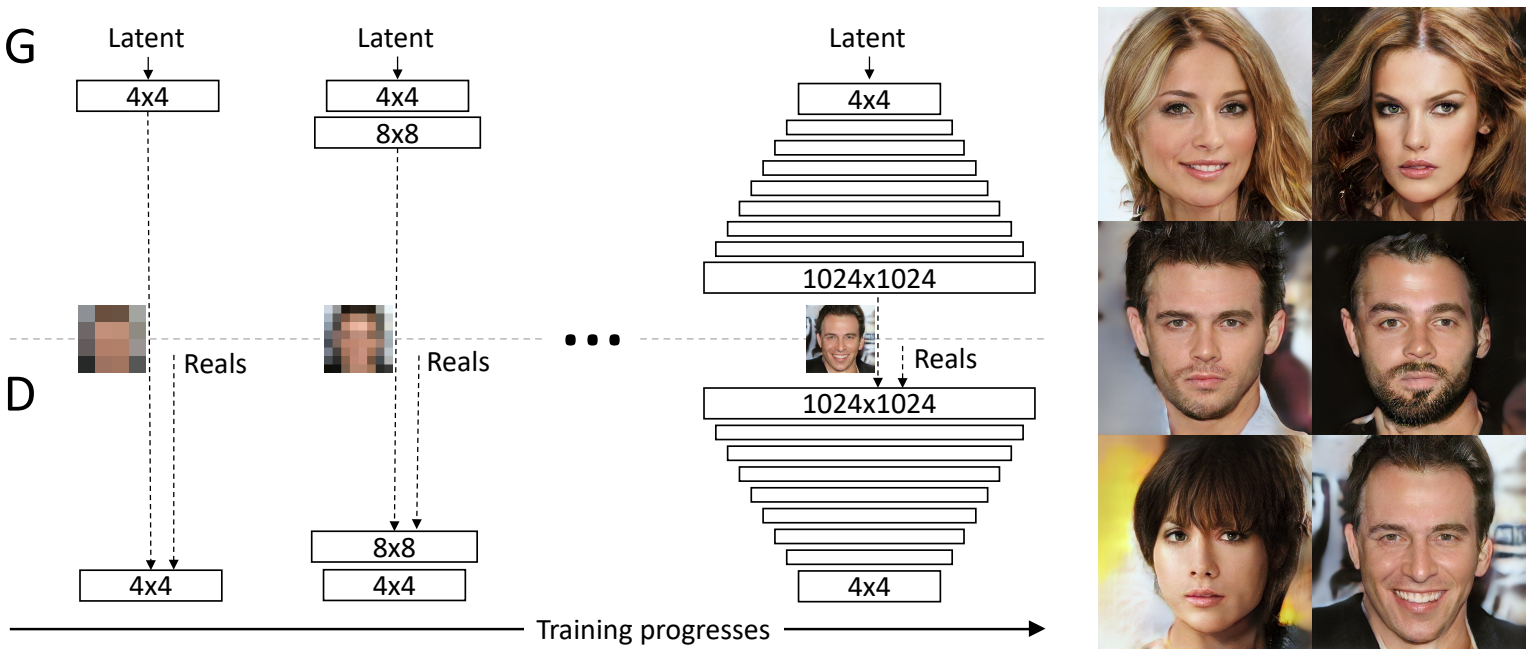
\includegraphics[width=0.8\linewidth]{figs/pggan_arch}
	\end{figure}
	\begin{figure}
		\centering
		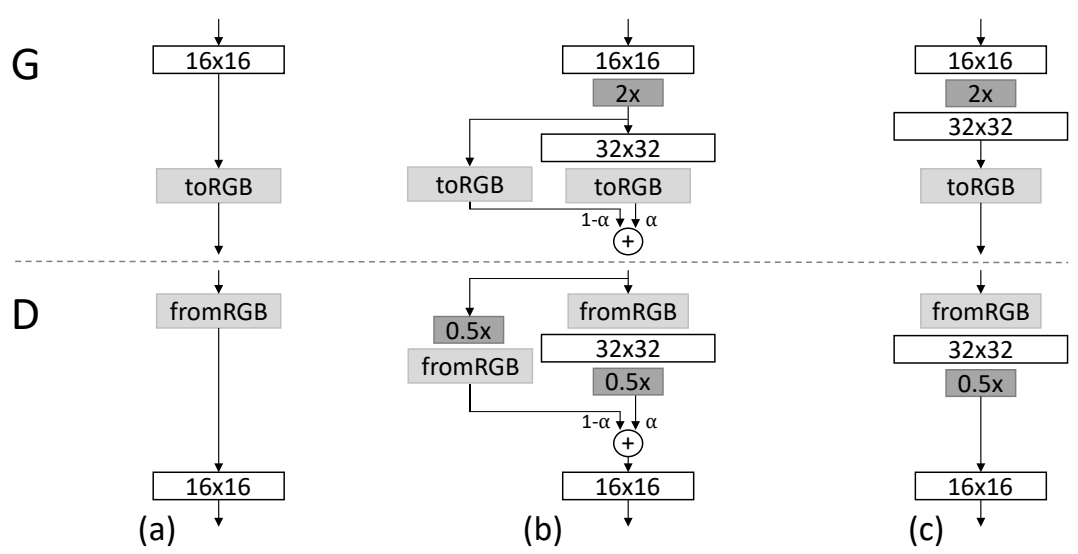
\includegraphics[width=0.6\linewidth]{figs/pggan_fadein}
	\end{figure}
	\vfill
	\hrule\medskip 
	{\scriptsize \href{https://arxiv.org/abs/1710.10196}{https://arxiv.org/abs/1710.10196}}
\end{frame}
%=======
\begin{frame}{Progressive Growing GAN}
	\begin{block}{Samples (1024x1024)}
		\begin{figure}
			\centering
			\includegraphics[width=\linewidth]{figs/pggan_samples}
		\end{figure}
	\end{block}
	\vfill
	\hrule\medskip 
	{\scriptsize \href{https://arxiv.org/abs/1710.10196}{https://arxiv.org/abs/1710.10196}}
\end{frame}
%=======
\begin{frame}{StyleGAN}
	\begin{itemize}
		\item Generating of HR images is hard.
		\item Progressive growing greatly simplifies the task.
		\item The ability to control specific features of the generated image is very limited.
	\end{itemize}
	\begin{block}{Face image features}
		\begin{itemize}
			\item Coarse (pose, general hair style, face shape). Resolution $4^2 - 8^2$.
			\item Middle (finer facial features, hair style, eyes open/closed). Resolution $16^2 - 32^2$.
			\item Fine (color scheme (eye, hair and skin) and micro features). Resolution $64^2 - 1024^2$.
		\end{itemize}
	\end{block}
	\vfill
	\hrule\medskip 
	{\scriptsize \href{https://arxiv.org/abs/1812.04948}{https://arxiv.org/abs/1812.04948}}
\end{frame}
%=======
\begin{frame}{StyleGAN}
	\begin{block}{Step 1: Mapping Network}
		\begin{itemize}
			\item Generator input is likely to be \textbf{disentangled}.  Each component of input vector $\bz$ should be responsible for one generative factor.
			\item Mapping network $f: \cZ \rightarrow \cW$ is used to reduce correlations between components of~$\bz$.
		\end{itemize}
		\begin{minipage}[t]{0.6\columnwidth}
			\begin{figure}
				\centering
				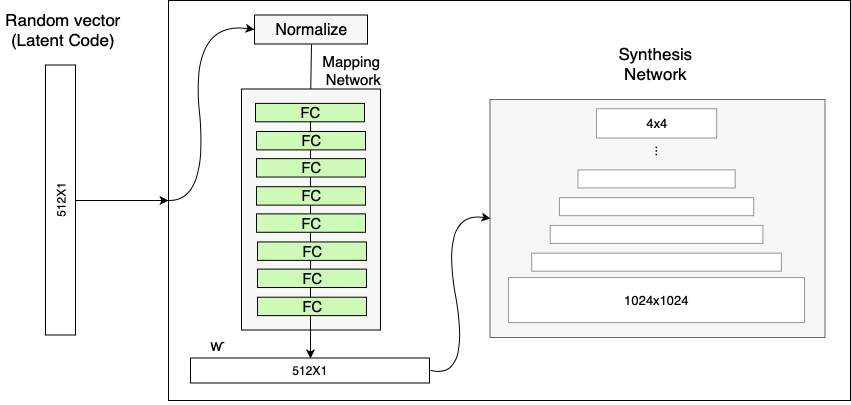
\includegraphics[width=0.98\linewidth]{figs/stylegan_mapping}
			\end{figure}
		\end{minipage}%
		\begin{minipage}[t]{0.38\columnwidth}
			\begin{figure}
				\centering
				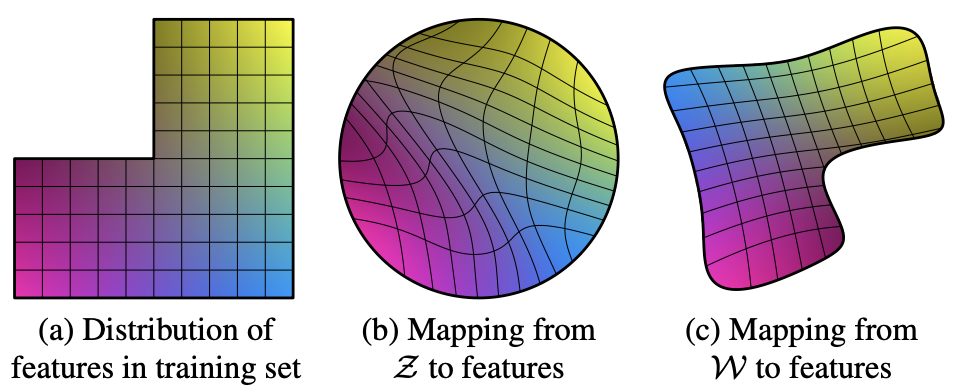
\includegraphics[width=1.0\linewidth]{figs/stylegan_curved}
			\end{figure}
		\end{minipage}
	\vspace{0.3cm}
	\end{block}
	\vfill
	\hrule\medskip 
	{\scriptsize \href{https://arxiv.org/abs/1812.04948}{https://arxiv.org/abs/1812.04948}}
\end{frame}
%=======
\begin{frame}{StyleGAN}
	\begin{block}{Step 2: Style modulation}
		\begin{itemize}
			\item Adaptive Instance Normalization transfers the $\bw$ vector to the synthesis Network.
			\item The module is added to each resolution to define the visual expression of the features.
		\end{itemize}
		\begin{figure}
			\centering
			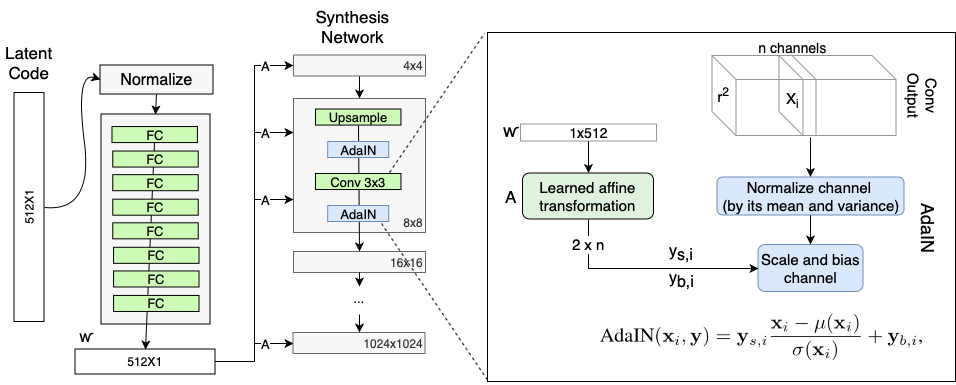
\includegraphics[width=1.0\linewidth]{figs/stylegan_adain}
		\end{figure}
	\end{block}
	\vfill
	\hrule\medskip 
	{\scriptsize \href{https://arxiv.org/abs/1812.04948}{https://arxiv.org/abs/1812.04948}}
\end{frame}
%=======
\begin{frame}{StyleGAN}
	\begin{block}{Step 3: Remove traditional input}
		Mapping network provides stochasticity to different stages of the synthesis network. Input of the synthesis network is a trainable vector.
		\begin{figure}
			\centering
			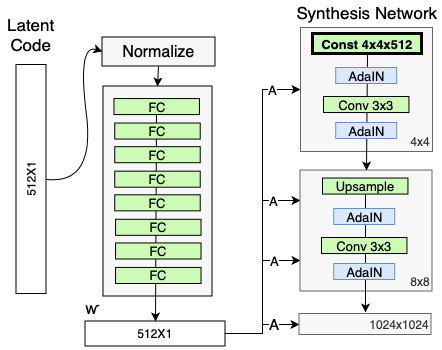
\includegraphics[width=0.55\linewidth]{figs/stylegan_input}
		\end{figure}
	\end{block}
	\vfill
	\hrule\medskip 
	{\scriptsize \href{https://arxiv.org/abs/1812.04948}{https://arxiv.org/abs/1812.04948}}
\end{frame}
%=======
\begin{frame}{StyleGAN}
	\begin{block}{Step 4: Stochastic variation}
		Inject random noise to add small aspects, such as freckles, exact placement of hairs, wrinkles, features which make the image more realistic and increase the variety of outputs.
		\begin{figure}
			\centering
			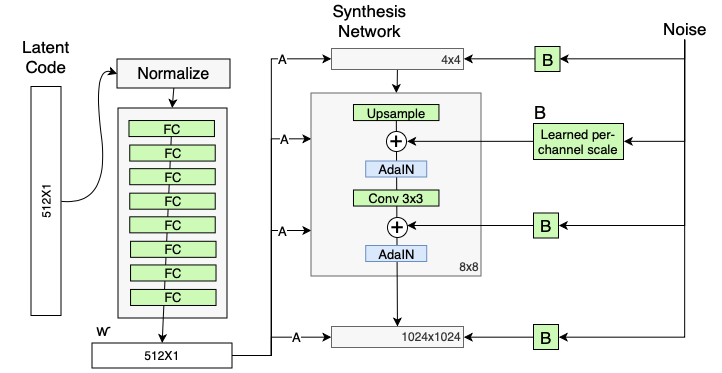
\includegraphics[width=0.9\linewidth]{figs/stylegan_noise}
		\end{figure}
	\end{block}
	\vfill
	\hrule\medskip 
	{\scriptsize \href{https://arxiv.org/abs/1812.04948}{https://arxiv.org/abs/1812.04948}}
\end{frame}
%=======
\begin{frame}{StyleGAN}
	\begin{block}{Step 4: Style Mixing}
		\vspace{-0.33cm}
		\begin{figure}
			\centering
			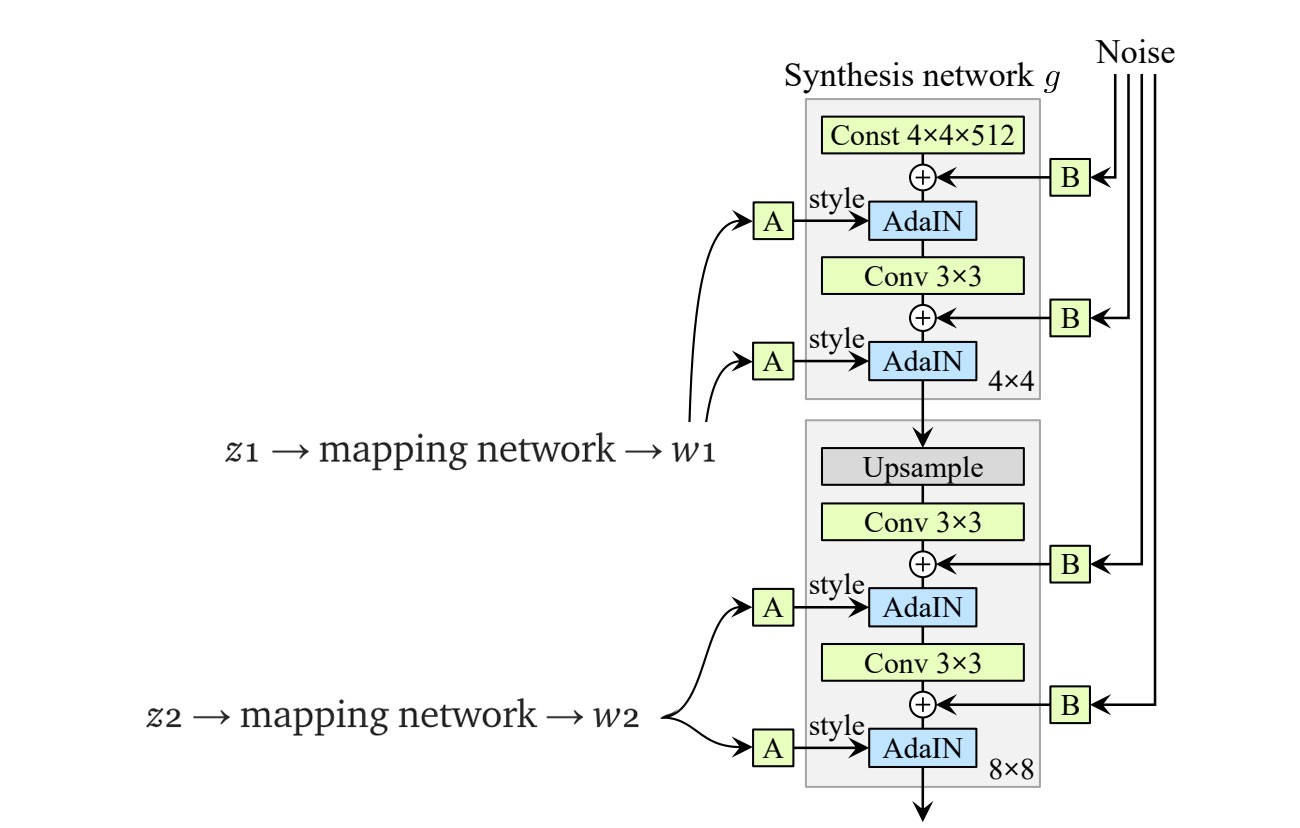
\includegraphics[width=0.8\linewidth]{figs/stylegan_mix_reg}
		\end{figure}
	\begin{itemize}
		\item Makes different levels of synthesis network to be independent.
		\item Allows to couple diffirent styles.
	\end{itemize}
	\end{block}
	\vfill
	\hrule\medskip 
	{\scriptsize \href{https://arxiv.org/abs/1812.04948}{https://arxiv.org/abs/1812.04948}}
\end{frame}
%=======
\begin{frame}{StyleGAN}
	\begin{figure}
		\centering
		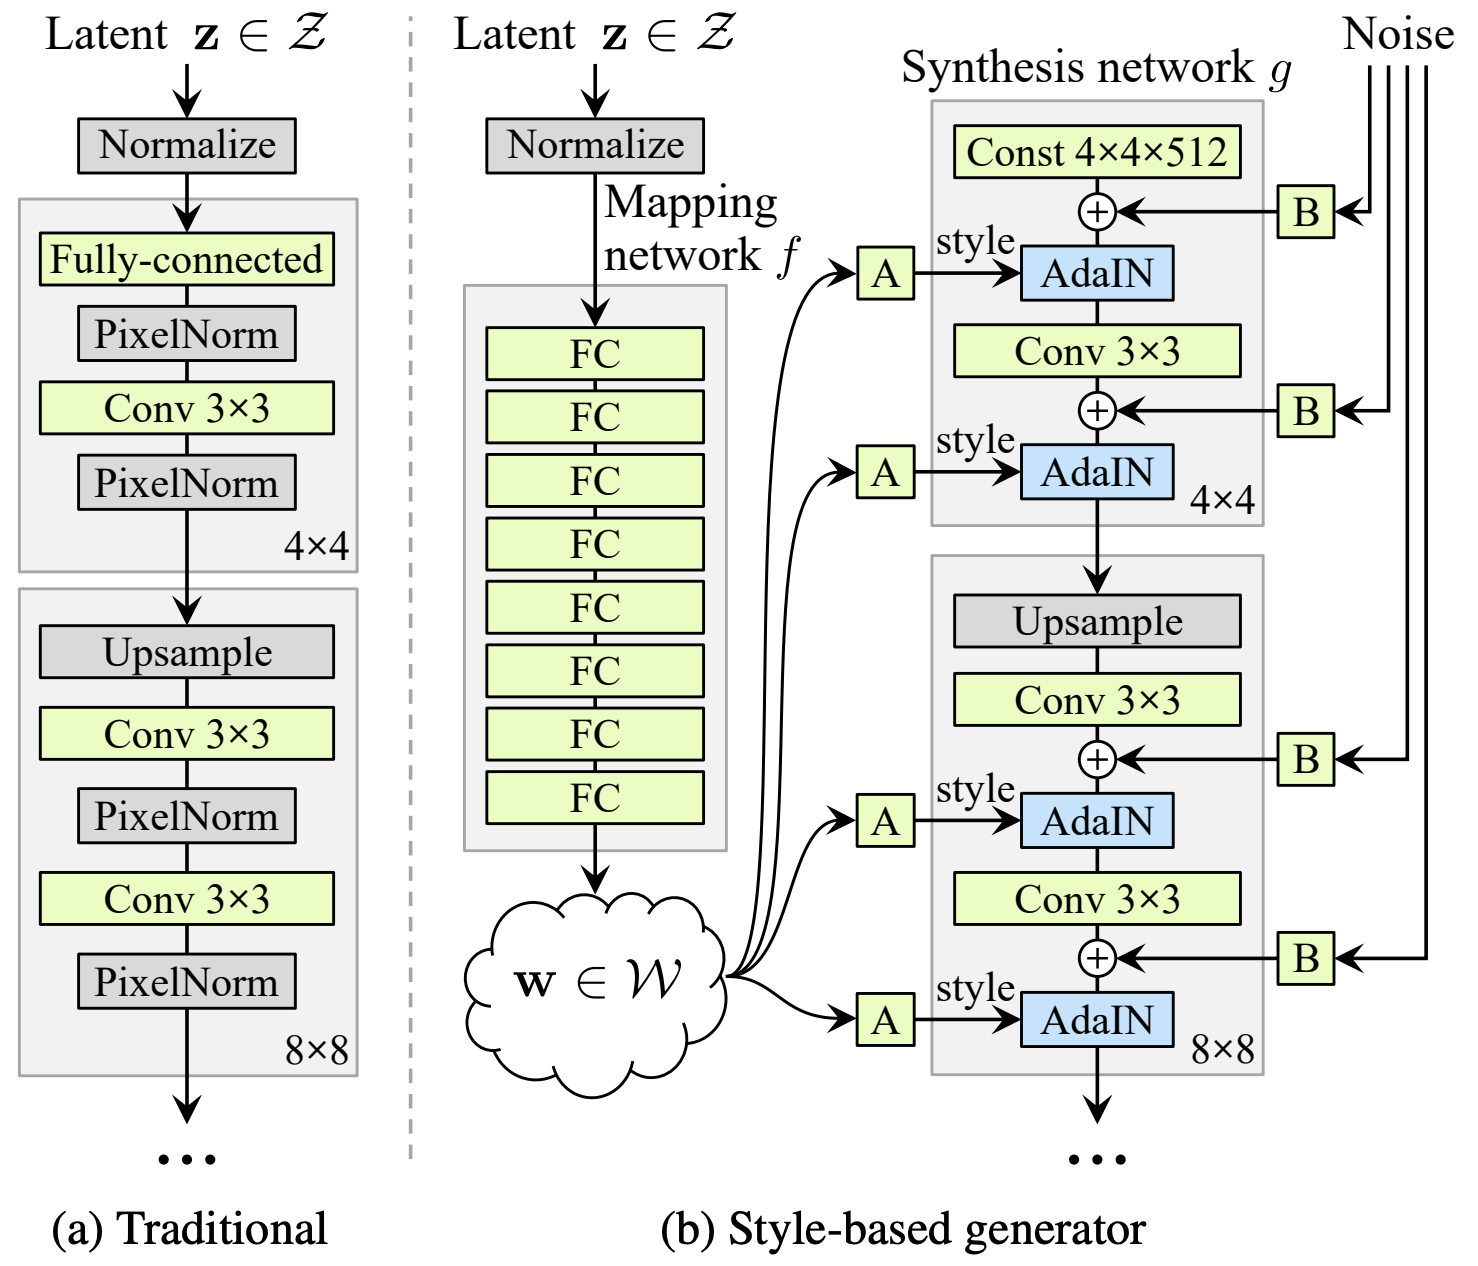
\includegraphics[width=0.8\linewidth]{figs/stylegan_scheme}
	\end{figure}
	\vfill
	\hrule\medskip 
	{\scriptsize \href{https://arxiv.org/abs/1812.04948}{https://arxiv.org/abs/1812.04948}}
\end{frame}
%=======
\begin{frame}{StyleGAN}
	\begin{block}{Truncation trick}
		\vspace{-0.2cm}
		\[
			\bw' = \hat{\bw} - \psi \cdot (\bw - \hat{\bw}), \quad \hat{\bw} = \bbE_{\bz} p(f(\bz))
		\]
		\vspace{-0.2cm}
		\begin{itemize}
			\item Constant $\psi$ is a tradeoff between diversity and fidelity. 
			\item $\psi=0.7$ is used for most of the results.
			\item Truncation is done only at the low-resolution layers.
		\end{itemize}
		\begin{figure}
			\centering
			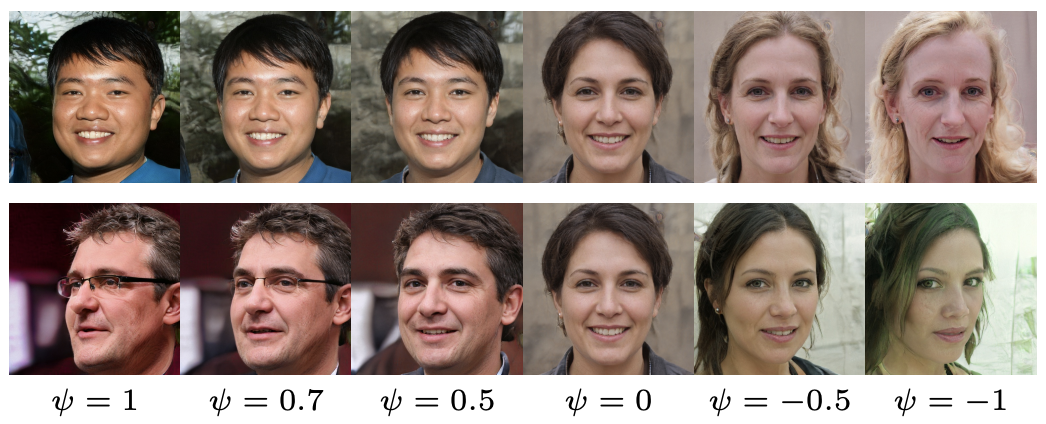
\includegraphics[width=0.8\linewidth]{figs/stylegan_truncation}
		\end{figure}
	\end{block}
	\vfill
	\hrule\medskip 
	{\scriptsize \href{https://arxiv.org/abs/1812.04948}{https://arxiv.org/abs/1812.04948}}
\end{frame}
%=======
\begin{frame}{StyleGAN}
	\begin{block}{Results}
		\vspace{-0.2cm}
		\begin{figure}
			\centering
			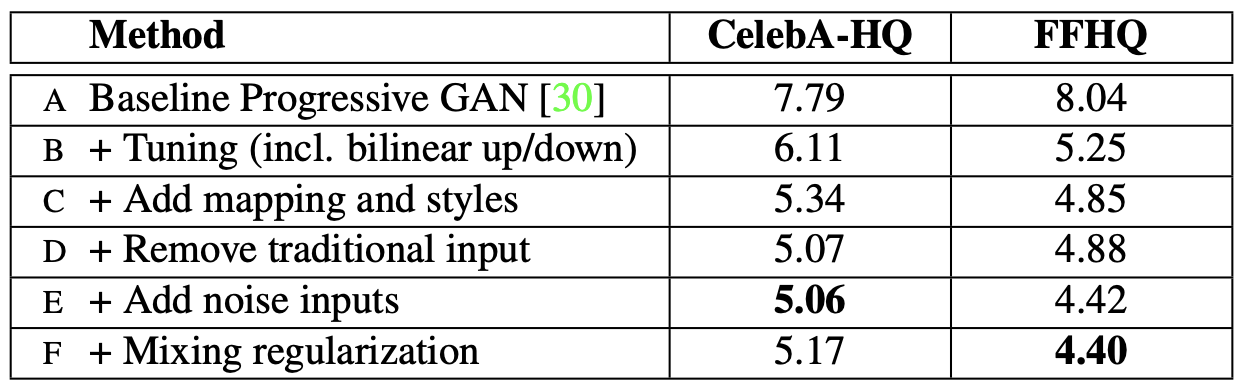
\includegraphics[width=0.6\linewidth]{figs/stylegan_results}
		\end{figure}
	\vspace{-0.3cm}
	\end{block}
	\begin{block}{Samples (1024x1024)}
		\begin{figure}
			\centering
			\includegraphics[width=0.8\linewidth]{figs/stylegan_samples}
		\end{figure}
	\vspace{-0.1cm}
	\end{block}
	\vfill
	\hrule\medskip 
	{\scriptsize \href{https://arxiv.org/abs/1812.04948}{https://arxiv.org/abs/1812.04948}}
\end{frame}
%=======
\begin{frame}{StyleGAN}
		\begin{figure}
			\centering
			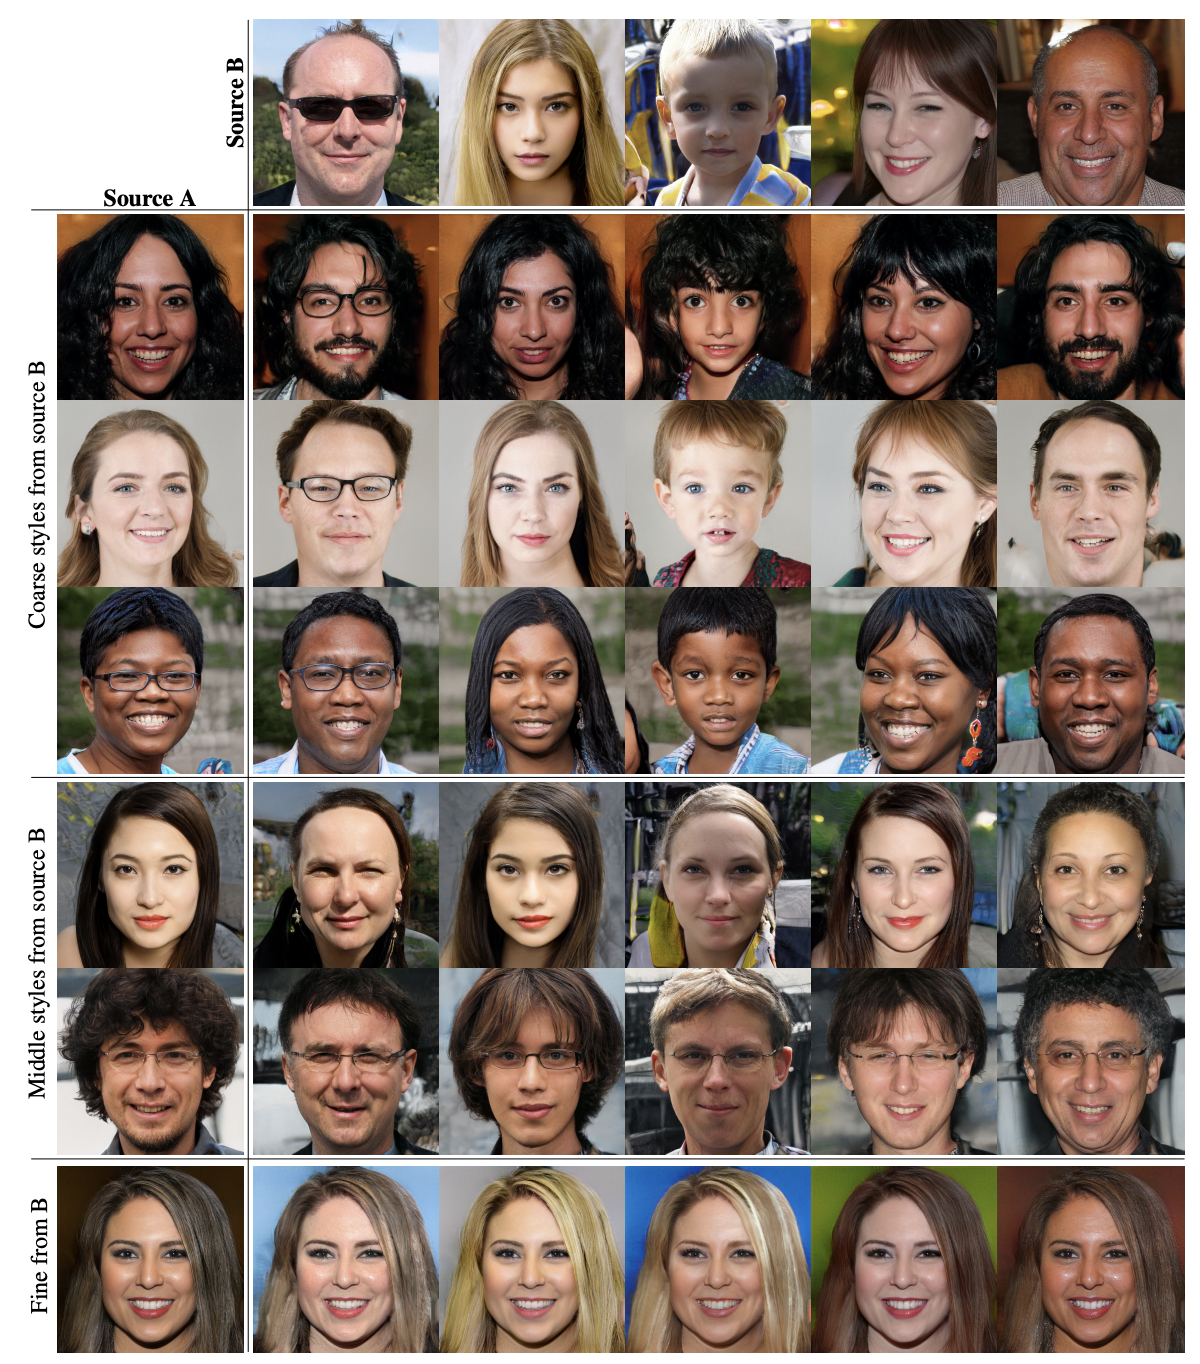
\includegraphics[width=0.6\linewidth]{figs/stylegan_mix}
		\end{figure}
	\vfill
	\hrule\medskip 
	{\scriptsize \href{https://arxiv.org/abs/1812.04948}{https://arxiv.org/abs/1812.04948}}
\end{frame}
%=======
\begin{frame}{References}
{\tiny
\begin{itemize}
	
	\item A Note on the Inception Score \\
	\href{https://arxiv.org/abs/1801.01973}{https://arxiv.org/abs/1801.01973} \\
	\textbf{Summary:} Inception Score is not an ideal metric.
	
	\item GANs Trained by a Two Time-Scale Update Rule Converge to a Local Nash Equilibrium \\
	\href{https://arxiv.org/abs/1706.08500}{https://arxiv.org/abs/1706.08500} \\
	\textbf{Summary:} Frechet inception distance was proposed for GAN evaluation.
	
	\item \textbf{SAGAN}: Self-Attention Generative Adversarial Networks \\
	\href{https://arxiv.org/abs/1805.08318}{https://arxiv.org/abs/1805.08318} \\
	\textbf{Summary:} Self-attention was proposed for G and D. Hinge loss was used for training. Spectral Normalization was injected \\
	not only for D, but also for G. 
	
	\item \textbf{BigGAN}: Large Scale GAN Training for High Fidelity Natural Image Synthesis \\
	\href{https://arxiv.org/abs/1809.11096}{https://arxiv.org/abs/1809.11096} \\
	\textbf{Summary:} SAGAN as a baseline. High-quality image generation. Increasing batch is really helpful (covering more modes). Propose orthogonalization regularization. Use truncation trick for trade-off between sample fidelity and variety.
	
	\item \textbf{ProGAN}: Progressive Growing of GANs for Improved Quality, Stability, and Variation \\
	\href{https://arxiv.org/abs/1710.10196}{https://arxiv.org/abs/1710.10196} \\
	\textbf{Summary:} The key idea is to grow both the generator and discriminator progressively: starting from a low resolution, \\
	we add new layers that model increasingly fine details as training progresses.
	
	\item \textbf{StyleGAN}: A Style-Based Generator Architecture for Generative Adversarial Networks  \\
	\href{https://arxiv.org/abs/1812.04948}{https://arxiv.org/abs/1812.04948} \\
	\textbf{Summary:} Mapping network for disentanglement. ProgressiveGAN as a baseline. AdaIN operation to modulate style. \\
	Noise injection for variability. Hierarchical style mixing. Perceptual path length as a measure of disentanglement.
\end{itemize}
}
\end{frame}
%=======
\end{document} 